\documentclass[onefignum, onetabnum]{siamart190516}
%\usepackage{natbib}
%\usepackage[sort]{cite}
\pdfoutput=1
%\usepackage[colorlinks=true,urlcolor=blue,citecolor=blue,linkcolor=blue]{hyperref}
\usepackage[english]{babel}
\usepackage[utf8]{inputenc}
\usepackage[T1]{fontenc}
\usepackage{amssymb}
\usepackage{tabularx}
\usepackage{quoting}
\usepackage{upquote}
\usepackage{subcaption}
\usepackage{multicol}
\usepackage{cancel}
\usepackage[framemethod=TikZ]{mdframed}
\usetikzlibrary{shapes}
\usetikzlibrary{snakes}
\usepackage{wrapfig}
%\usepackage{caption}
%\usepackage[plain]{algorithmic}
\usepackage[linesnumbered, ruled, vlined, algo2e]{algorithm2e}
\usepackage{algpseudocode}
\usepackage{rotating}
%\usepackage{cite}
\usepackage{booktabs}
%\usepackage{unicode-math}
%\usepackage{algorithm}% http://ctan.org/pkg/algorithm
%\usepackage{algpseudocode}% http://ctan.org/pkg/algpseudocode
\usepackage{xcolor}% http://ctan.org/pkg/xcolor
\makeatletter
\newsavebox{\@brx}
\newcommand{\llangle}[1][]{\savebox{\@brx}{\(\m@th{#1\langle}\)}%
  \mathopen{\copy\@brx\kern-0.5\wd\@brx\usebox{\@brx}}}
\newcommand{\rrangle}[1][]{\savebox{\@brx}{\(\m@th{#1\rangle}\)}%
  \mathclose{\copy\@brx\kern-0.5\wd\@brx\usebox{\@brx}}}
\makeatother
\usepackage{bbm}
\usepackage{jlcode}
\usepackage{graphicx}
\usepackage{amsmath,color}
\usepackage{mathrsfs}
\usepackage{float}
\usepackage[normalem]{ulem}
\usepackage{makecell}
\usepackage{indentfirst}
\usepackage{txfonts}
%\usepackage[epsilon, tsrm, altpo]{backnaur}

\makeatletter
\def\parsept#1#2#3{%
    \def\nospace##1{\zap@space##1 \@empty}%
    \def\rawparsept(##1,##2){%
        \edef#1{\nospace{##1}}%
        \edef#2{\nospace{##2}}%
    }%
    \expandafter\rawparsept#3%
}
\makeatother
\DeclareMathAlphabet{\mymathbb}{U}{BOONDOX-ds}{m}{n}
\newcommand{\listingcaption}[1]%
{%
\refstepcounter{lstlisting}\hfill%
Listing \thelstlisting: #1\hfill%\hfill%
}%
\newcolumntype{b}{X}
\newcolumntype{s}{>{\hsize=.7\hsize}X}
\usepackage{listings}
\lstset{
    language=Julia,
    basicstyle=\ttfamily\scriptsize,
    numberstyle=\scriptsize,
    % numbers=left,
    backgroundcolor=\color{gray!7},
    %backgroundcolor=\color{white},
    %frame=single,
    xleftmargin=2em,
    tabsize=2,
    rulecolor=\color{black!15},
    %title=\lstname,
    escapeinside={(*}{*)},
    breaklines=true,
    %breakatwhitespace=true,
    %framextopmargin=2pt,
    %framexbottommargin=2pt,
    frame=bt,
    extendedchars=true,
    inputencoding=utf8,
    columns=fullflexible,
    %escapeinside={(*@}{@*)},
}

\tolerance=1
\emergencystretch=\maxdimen
\hyphenpenalty=1000
\hbadness=1000

\makeatletter

%%%%%%%%%%%%%%%%%%%%%%%%%%%%%% User specified LaTeX commands.

%Journal reference.  Comma sets off: name, vol, page, year
\def\journal #1, #2, #3, 1#4#5#6{{\sl #1~}{\bf #2}, #3 (1#4#5#6) }
\def\pr{\journal Phys. Rev., }
\def\prb{\journal Phys. Rev. B, }
\def\prl{\journal Phys. Rev. Lett., }
\def\pl{\journal Phys. Lett., }
%\def\np{\journal Nucl. Phys., }


%%%%%%%%%%%%%%%%%%%%%%%%%%%%%%%%%%%%%%%%%%%%%%%%%%%%%%%%%%%%%%%%%%%%%%%%%%%%%%%%%%%%%%%%%%%%%%%%%%%%%%%%%%%%%%%%%%%%%%%%%%%%%%%%%%%%%%%%%%%%%%%%%%%%%%%%%%%%%%%%%%%%%%%%%%%%%%%%%%%%%%%%%%%%%%%%%%%%%%%%%%%%%%%%%%%%%%%%%%%%%%%%%%%%%%%%%%%%%%%%%%%%%%%%%%%%


%\usepackage{CJK}
%\usepackage[colorlinks, citecolor=blue]{hyperref}
\DeclareMathOperator*{\argmax}{arg\,max}

%%%%%% Shortcut related
\newcommand{\<}{\langle}
\renewcommand{\>}{\rangle}
\newcommand{\out}{{\vx^L}}
\newcommand{\inp}{{\vx^0}}
\newcommand{\cquad}{{{ }_{\quad}}}
\newcommand{\pluseq}{\mathrel{+}=}
\newcommand{\minuseq}{\mathrel{-}=}
\newcommand{\vx}{{\mathbf{x}}}
\newcommand{\vg}{{\mathbf{g}}}
\newcommand{\vp}{{\mathbf{p}}}
\newcommand{\vy}{{\mathbf{y}}}
\newcommand{\Var}{{\mathrm{Var}}}
\newcommand{\Mean}{{\mathrm{E}}}
\newcommand{\vvalue}{{\texttt{value}}}
\newcommand{\grad}{{\texttt{grad}}}
\newcommand{\parameter}{{\texttt{parameter}}}
%%%%%% Convention related
\newcommand{\SWAP}{{\rm SWAP}}
\newcommand{\CNOT}{{\rm CNOT}}
\newcommand{\bigO}{{\mathcal{O}}}
\newcommand{\X}{{\rm X}}
\renewcommand{\H}{{\rm H}}
\newcommand{\Rx}{{\rm Rx}}
\renewcommand{\v}[1]{{\bf #1}}
\newcommand{\dataset}{{\mathcal{D}}}
\newcommand{\wfunc}{{\psi}}
\newcommand{\SU}{{\rm SU}}
\newcommand{\UU}{{\rm U}}
\newcommand{\thetav}{{\boldsymbol{\theta}}}
\newcommand{\gammav}{{\boldsymbol{\gamma}}}
\newcommand{\thetai}{{\theta^\alpha_l}}
\newcommand{\Expect}{{\mathbb{E}}}
\newcommand{\Tr}{{\rm Tr}}
\newcommand{\etc}{{\it etc~}}
\newcommand{\etal}{{\it etal~}}
\newcommand{\xset}{\mathbf{X}}
\newcommand{\fl}{\texttt{fl}}
\newcommand{\pdata}{\mathbf{\pi}}
\newcommand{\q}{\mathbf{q}}
\newcommand{\epdata}{\mathbf{\hat{\pi}}}
\newcommand{\gammaset}{\boldsymbol{\Gamma}}
\newcommand{\ei}{{\mathbf{e}_l^\alpha}}
\newcommand{\vtheta}{{\boldsymbol{\theta}}}
\newcommand{\sigmag}{{\nu}}
\newcommand{\sigmai}[2]{{\sigma^{#2}_{#1}}}
\newcommand{\qi}[1]{{q^{\alpha_{#1}}_{#1}}}
\newcommand{\BAS}{Bars-and-Stripes}
\newcommand{\circled}[1]{\raisebox{.5pt}{\textcircled{\raisebox{-.9pt} {#1}}}}
\newcommand{\qexpect}[1]{{\left\langle #1\right\rangle}}
\newcommand{\expect}[2]{{\mathop{\mathbb{E}}\limits_{\substack{#2}}\left[#1\right]}}
\newcommand{\var}[2]{{\mathop{\mathrm{Var}}\limits_{\substack{#2}}\left(#1\right)}}
\newcommand{\pshift}[1]{{p_{\thetav+#1}}}
\newcommand{\upcite}[1]{\textsuperscript{\cite{#1}}}
\newcommand{\Eq}[1]{Eq.~(\ref{#1})}
\newcommand{\Fig}[1]{Fig.~\ref{#1}}
\newcommand{\Lst}[1]{Listing.~\ref{#1}}
\newcommand{\Tbl}[1]{Table~\ref{#1}}
\newcommand{\Sec}[1]{Sec.~\ref{#1}}
\newcommand{\App}[1]{Appendix~\ref{#1}}
\newcommand{\bra}[1]{\mbox{$\left\langle #1 \right|$}}
\newcommand{\ket}[1]{\mbox{$\left| #1 \right\rangle$}}
\newcommand{\braket}[2]{\mbox{$\left\langle #1 | #2 \right\rangle$}}
\newcommand{\tr}[1]{\mathrm{tr}\mbox{$\left[ #1\right]$}}

\newcommand{\ra}[1]{\renewcommand{\arraystretch}{#1}}

%%%%%% Comment related
\newcommand{\red}[1]{[{\bf  \color{red}{ST: #1}}]}
\newcommand{\xred}[1]{[{\bf  \color{red}{\sout{ST: #1}}}]}
\newcommand{\green}[1]{[{\bf  \color{green}{XG: #1}}]}
\newcommand{\xgreen}[1]{[{\bf  \color{green}{\sout{XG: #1}}}]}
\newcommand{\blue}[1]{[{\bf  \color{blue}{JG: #1}}]}
\newcommand{\xblue}[1]{[{\bf  \color{blue}{\sout{JG: #1}}}]}
\newcommand{\material}[1]{\iffalse[{\bf  \color{cyan}{Material: #1}}]\fi}

\newcounter{example}
\newenvironment{example}[1][]{\refstepcounter{example}\par\medskip
   \noindent \textbf{Example~\theexample. #1} \rmfamily}{\medskip}

%\newtheorem{theorem}{\textit{Theorem}}
%\newtheorem{corollary}{\textit Branching Rule}
%\theoremstyle{definition}\newtheorem{definition}{\textit{Definition}}
%\newtheorem{defin}[thm]{Definition}

\makeatother

%\externaldocument{ex_supplement}

\title{Computing properties of independent sets by generic programming tensor networks
\thanks{\funding{...}}
}

\author{XXX\thanks{XXX 
  (\email{email}, \url{website}).}
\and YYY\thanks{yyyyy 
  (\email{yyyy}, \email{email}).}
}

\begin{document}

\maketitle

\begin{abstract}
We introduce a new approach to compute various properties of independent sets by encoding the problems and the graph into tensor networks with different tensor element algebra.
The type of graph problems that can be computed using this method includes: independence number, the number of independent sets, independence polynomial, maximal independence polynomial, and both counting and enumeration of all maximum independence sets, the large-size independent sets, and all maximal independent sets.
Although the computational complexity inevitably scales exponentially with the graph size, our method using tensor network contraction with generic programming is highly versatile and is able to compute properties that are otherwise not known to be possible for up to several hundred vertices.
At the same time, our algorithms are very simple to implement and one can directly utilize recent advances in tensor network contraction techniques.
To demonstrate the versatility of this tool, we apply it to a few examples including the calculations of the hard-square entropy constant, Euler characteristics of the independence complex, partition functions, and finite-temperature phase transitions on square-lattice graphs.
\end{abstract}

% REQUIRED
\begin{keywords}
independent set, tensor network, maximum independent set, independence polynomial
\end{keywords}

% REQUIRED
% 14N07  	Secant varieties, tensor rank, varieties of sums of powers
\begin{AMS}
  05C31, 14N07
\end{AMS}

\section{Introduction}
\blue{overlap gap property~\cite{Gamarnik2013, Gamarnik2019}, independence polynomial at -1~\cite{Bousquet2008,Levit2009},
branching algorithm~\cite{Tarjan1977,Robson1986},
two motivations of computing independence polynomial: 1. Lee-Yang zero~\cite{Lee1952,Yang1952}, 2. Lov{\'a}sz local lemma~\cite{Scott2005}.
}
In graph theory and combinatorics, there are many interesting but hard computational problems concerning properties of independent sets.
An independent set is a set of vertices in a graph where no two vertices are adjacent to each other.
More formally, given an undirected graph $G = (V,E)$, an independent set $I \subseteq V$ is a set that for any $u,v \in I$, there is no edge connecting $u$ and $v$ in $G$.
The problem of finding an independent set of the largest possible size, the maximum independent set (MIS), is a paradigmatic NP-complete problem~\cite{Hastad1996}.
The size of the MIS of a graph $G$ is called the independence number, denoted as $\alpha(G) \equiv \max_{I}|I|$. 

Finding $\alpha(G)$ is a hard computational problem; moreover, it is NP-hard to even approximate $\alpha(G)$ within a factor $|V|^{1-\epsilon}$ for an arbitrarily small positive $\epsilon$.
Naive exhaustive search for the MIS requires time $O\left(2^{|V|} \right)$. More efficient exact algorithms include the branching algorithms and dynamic programming.
Sophisticated branching algorithms can reduce the base of the exponential time scaling to, e.g., $1.1996^{|V|} {|V|}^{O(1)}$~\cite{Xiao2017}.
Dynamic programming approaches~\cite{Courcelle1990, Fomin2013} works better for graphs with a small treewidth $\text{tw}(G)$;
these methods can produce algorithms of complexity $O(2^{\text{tw}(G)} \text{tw}(G) |V|)$.

The independent set problem is closely related to the clique problem and the vertex cover problem~\cite{Moore2011};
more concretely, an MIS of a graph $G$ corresponds to a maximum clique in the complement graph of $G$,
and the complement vertex set of an MIS corresponds to a minimum vertex cover of the graph $G$.
Together, these problems find a wide range of applications in scheduling, logistics, social network analysis, bioinformatics, wireless networks and telecommunication,
map labelling, computer vision, etc.~\cite{Butenko2003, Wu2015}.
Besides the standard problem of finding the independence number and an MIS, there are many other interesting problems pertaining to independent sets, such as the number of independent sets,
independence polynomial, maximal independence polynomial, and enumeration of MIS or maximal independent set configurations.
Some of these problems are of great interest in physics applications such as the hard-core lattice gas model~\cite{Dyre2016, Fernandes2007}
in statistical mechanics and the Rydberg hamiltonian with neutral atoms~\cite{Pichler2018} \red{cite experiment when it's ready};
they can, for example, be used to understand phase transitions and to identify harder graphs in an ensemble of graphs \red{cite experiment}.

In this work, we introduce a tensor-network based framework to compute the various properties pertaining to independent sets.
We map different problems into generic tensor network contraction with various tensor element algebra.
Our approach does not necessarily provide a better time complexity compared to dynamic programming,
but the tensor network approach is highly versatile so different problems can be generically solved with minimal implementation efforts without loss of efficiency.
We benchmark our algorithms by computing various independent set properties on CPUs and GPUs, the implementation of which benefits from recent advances in tensor-network contraction for the purposes of quantum circuit simulations~\cite{Gray2021, Pan2021}.
Lastly, we provide a few examples and show that the toolbox can be used to calculate the hard-square entropy constant,
Euler characteristics of the independence complex, partition functions, and finite-temperature phase transitions on square-lattice graphs. 

\section{Tensor networks}
A tensor network~\cite{Cirac2020, Orus2014} can be viewed as a generalization of matrix multiplication to multi-dimensional tensor contraction.
Let $A, B$ be two matrices; the matrix multiplication is defined as $C_{ik} = \sum_{j}A_{ij}B_{jk}$.
Using the Einstein notation, we can write $C_{ik} = A_{ij}B_{jk}$, where $j$ is implicitly summed over.
In the standard notation, each index can appear at most twice. A tensor network consists of multiple tensors performing the sum-product operation,
i.e., contraction, and the tensor network can be represented as a multigraph with open edges by viewing a tensor as a vertex,
a label pairing two tensors as an edge, and the remaining unpaired labels as open edges.

\begin{example}
   A tensor network $C_{il} = A_{ijkm} B_{kml} V_{j}$ has the following multigraph representation.
   
\centerline{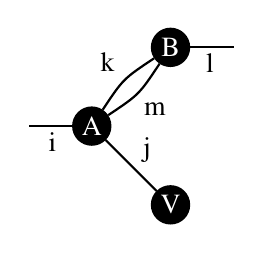
\begin{tikzpicture}[
    dot/.style = {circle, fill, minimum size=#1,
                inner sep=0pt, outer sep=0pt},
    dot/.default = 6pt  % size of the circle diameter 
                    ]
    \def\dx{0};
    \def\r{0.25cm}
    \def\ax{0}
    \def\ay{0}
    \def\bx{1}
    \def\by{1}
    \def\cx{1}
    \def\cy{-1}
    \node[color=white, fill=black, dot=2*\r] at (\ax+\dx,\ax) (a) {A};
    \node[color=white, fill=black, dot=2*\r] at (\bx+\dx,\by) (b) {B};
    \node[color=white, fill=black, dot=2*\r] at (\cx+\dx,\cy) (c) {V};
    %\draw [black,thick] (\ax+\dx,\ay) .. controls (0.5*\ax+0.5*\bx+\dx+0.2,0.5*\ay+0.5*\by-0.2) .. (\bx+\dx,\by);
    %\draw [black,thick] (\ax+\dx,\ay) .. controls (0.5*\ax+0.5*\bx+\dx-0.2,0.5*\ay+0.5*\by+0.2) .. (\bx+\dx,\by);
    \draw [black,thick] (a) .. controls (0.4, 0.6) .. (b);
    \draw [black,thick] (a) .. controls (0.6, 0.4) .. (b);
    \draw [black,thick] (a) -- (c);
    \draw [black,thick] (a) -- (\ax+\dx-0.8,\ay);
    \draw [black,thick] (b) -- (\bx+\dx+0.8,\by);
    \node[color=black] at (0.5*\ax+0.5*\bx-0.3+\dx,0.5*\ay+0.5\by+0.3) {k};
    \node[color=black] at (0.5*\ax+0.5*\bx+0.3+\dx,0.5*\ay+0.5\by-0.3) {m};
    \node[color=black] at (0.5*\ax+0.5*\cx+\dx+0.2,0.5*\ay+0.5\cy+0.2) {j};
    \node[color=black] at (\ax+\dx-0.5,\ay-0.2) {i};
    \node[color=black] at (\bx+\dx+0.5,\by-0.2) {l};
\end{tikzpicture}}
\end{example}

One can generalize the tensor network notation by removing the restriction that each index can appear at most twice.
The notation can be considered as a generalized Einstein notation, which is sometimes called einsum,
sum-product network or factor graph~\cite{Bishop2006} in different contexts.
The graphical representation of a tensor network we use in this paper is a hypergraph, where an edge (label) can be shared by an arbitrary number of vertices (tensors).

\begin{example}
$C_{ijk} = A_{jkm} B_{mil} V_{jm}$ is a tensor network representing $C_{ijk} = \sum_{ml}A_{jkm} B_{mil} V_{jm}$,
where $i,j,k$ in the output tensor are open edges (note that $j$ is not an open edge and thus summed over).
Its hypergraph representation is shown below, where we use different colors to annotate different hyperedges.

\centerline{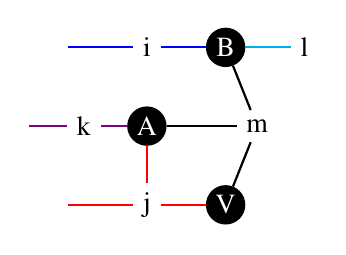
\begin{tikzpicture}[
    dot/.style = {circle, fill, minimum size=#1,
                inner sep=0pt, outer sep=0pt},
    dot/.default = 6pt  % size of the circle diameter 
                    ]  
    \def\dx{0};
    \def\r{0.5cm}
    \def\sr{0.15cm}
    \def\ax{0}
    \def\ay{0}
    \def\bx{1}
    \def\by{1}
    \def\cx{1}
    \def\cy{-1}
    \node[color=white,fill=black,dot=\r] at (\ax+\dx,\ax) (a) {A};
    \node[color=white,fill=black,dot=\r] at (\bx+\dx,\by) (b) {B};
    \node[color=white,fill=black,dot=\r] at (\cx+\dx,\cy) (v) {V};
    \node[color=transparent,draw=transparent,dot=0] at (\ax-1,\by) (o1) {};
    \node[color=transparent,draw=transparent,dot=0] at (\ax-1.5,\ay) (o2) {};
    \node[color=transparent,draw=transparent,dot=0] at (\ax-1,\cy) (o3) {};
    \node at (\ax-0.8,\ay) (k) {k};
    \node at (\bx+0.4,\ay) (m) {m};
    \node at (\ax,\cy) (j) {j};
    \node at (\bx+1,\by) (l) {l};
    \node at (\bx-1,\by) (i) {i};
    \draw[color=blue,thick] (i) -- (b);
    \draw[color=blue,thick] (i) -- (o1);
    \draw[color=cyan,thick] (l) -- (b);
    \draw[color=violet,thick] (k) -- (a);
    \draw[color=violet,thick] (k) -- (o2);
    \draw[color=black,thick] (b) -- (m);
    \draw[color=black,thick] (m) -- (a);
    \draw[color=black,thick] (m) -- (v);
    \draw[color=red,thick] (a) -- (j);
    \draw[color=red,thick] (v) -- (j);
    \draw[color=red,thick] (o3) -- (j);
\end{tikzpicture}}
\end{example}

In the main text, we use the generalized tensor network notation. The generalized tensor network can be easily translated to the standard notation by adding identity tensors denoted as $\delta$ tensors.
The example above can be written as $C_{ijk} = A_{jkm} B_{mil} V_{jm} = A_{ukm} B_{pil} V_{vq} \delta_{mpq} \delta_{juv}\delta_l$ in the standard notion. However, by adding the $\delta$ tensors, one may unnecessarily increase the contraction complexity of a graph, which we illustrate in \App{app:tensorbad}.

\section{Generic programming}\label{sec:generic}
In previous works relating tensor networks and combinatoric problems~\cite{Kourtis2019, Biamonte2017},
the elements in the tensor networks are limited to standard number types such as floating point numbers and integers.
Owning to the development of modern compiling technology, we no longer need to limit our imagination to standard number types.
One of the key concepts that push the technology forward is called generic programming:

\begin{definition}[Generic programming]
   Generic programming is an approach to programming that focuses on designing algorithms and data structures so that they work in the most general setting without loss of efficiency. ~\cite{Stepanov2014}
\end{definition}

This definition of generic programming contains two major aspects: a single program for the general setting and efficiency.
To understand the first aspect, suppose we want to write a function that raises an element to a power, $f(x, n) := x^n$.
One can easily write a function for standard number types that computes the power of $x$ in $\log(n)$ steps using the multiply and square trick.
Generic programming does not require $x$ to be a standard number type,
instead it treats $x$ as an element with an associative multiplication operation $\odot$ and a multiplicative identity $\mymathbb{1}$.
In such a way, when the program takes a matrix as an input, it computes the matrix power without extra efforts.
The second aspect is about performance. For dynamically typed languages such as Python,
one can easily write very general codes, but the efficiency is not guaranteed; for example, the speed of computing the matrix multiplication between two numpy arrays with python objects as elements is much slower than statically typed languages such as C++ and Julia~\cite{Bezanson2012}.
C++ uses templates for generic programming while Julia takes advantage of just-in-time compilation and multiple dispatch.
When these languages ``see'' a new input type, the compiler can recompile the generic program for the new type.
A myriad of optimizations can be done during the compilation, such as inlining immutable elements with fixed sizes in an array to decrease the cache miss rate when accessing data.
In Julia, these inlined arrays can even be compiled to GPU devices for faster computation~\cite{Besard2018}.

This motivates us to think about what is the most general element type that is allowed in a tensor network contraction program.
We find that as long as the algebra of tensor elements forms a commutative semiring, the tensor network contraction result will be valid and be independent of the contraction order.
A commutative semiring is a semiring with its multiplication operation being commutative, while a semiring is a ring without additive inverse.
To define a commutative semiring with the addition operation $\oplus$ and the multiplication operation $\odot$ on a set $R$, the following relations must hold for any arbitrary three elements $a, b, c \in R$.
\begin{align*}
(a \oplus b) \oplus c = a \oplus (b \oplus c) & \hspace{5em}\text{$\triangleright$ commutative monoid $\oplus$ with identity $\mymathbb{0}$}\\
a \oplus \mymathbb{0} = \mymathbb{0} \oplus a = a &\\
a \oplus b = b \oplus a &\\
&\\
(a \odot b) \odot c = a \odot (b \odot c)  &   \hspace{5em}\text{$\triangleright$ commutative monoid $\odot$ with identity $\mymathbb{1}$}\\
a \odot  \mymathbb{1} =  \mymathbb{1} \odot a = a &\\
a \odot b = b \odot a &\\
&\\
a \odot (b\oplus c) = a\odot b \oplus a\odot c  &  \hspace{5em}\text{$\triangleright$ left and right distributive}\\
(a\oplus b) \odot c = a\odot c \oplus b\odot c &\\
&\\
a \odot \mymathbb{0} = \mymathbb{0} \odot a = \mymathbb{0}
\end{align*}
The requirement of being commutative is for the tensor contraction result to be independent of the contraction order, which could be relaxed in certain cases. In the following sections, we show how to compute the independence polynomial,
the maximal independence polynomial, independence number, the number of independent sets, and enumeration of the MIS and maximal independent set configurations of a general graph $G$ by designing tensor element types as commutative semirings while keeping the tensor network generic~\cite{Stepanov2014}.
Table~\ref{tbl:generictypes} summarizes the problems that can be solved by various tensor element types. 

\begin{table}[t!]\centering
\begin{minipage}{\columnwidth}
\ra{1.3}
        \begin{tabularx}{\textwidth}{bb}\toprule
            \hline
            \textbf{element type}     & \textbf{purpose} \\
            {real number}     & {counting all independent sets} \\
            {tropical number} (\Eq{eq:countingtropical})    & {finding the independence number} \\
            {tropical number with counting} (\Eq{eq:countingtropical})     & {finding the independence number and the number of MISs} \\
            {tropical number with configurations} (\Eq{eq:singleconfig})     & {finding the independence number and one MIS} \\
            {tropical number with sets} (\Eq{eq:countingtropicalset})    & {finding the independence number and enumeration of all MISs} \\
            {polynomial} (\Eq{eq:polynomial})     & {computing the independence polynomial exactly} \\
            {truncated polynomial} (\Eq{eq:max2poly})     & {counting MISs and independent sets of size $\alpha(G)-1$} \\
            {complex number}     & {fitting the independence polynomial with fast Fourier transform} \\
            {finite-field algebra (\Eq{eq:finitefield})} & {fitting the independence polynomial exactly using number theory} \\
            \bottomrule
        \end{tabularx}
    \caption{Tensor element types and their purposes in calculating various independent set properties.}\label{tbl:generictypes}
\end{minipage}
\end{table}

\section{Independence polynomial and maximal independence polynomial}
\subsection{Independence polynomial}\label{sec:indpoly}
The independence polynomial is an important graph polynomial that contains the counting information of independent sets. It is defined as
\begin{equation}
I(G, x) = \sum_{k=0}^{\alpha(G)} a_k x^k,
\end{equation}
where $a_k$ is the number of independent sets of size $k$ in $G$, and $\alpha(G)$ is the independence number. The total number of independent sets is thus equal to $I(G, 1)$.
The problem of computing the independence polynomial belongs to the complexity class \#P-hard. One approach to exactly compute the independence polynomial requires a computational time of $O(1.442^{|V|})$~\cite{Ferrin2014}
\blue{I am not sure about this complexity, this is based on the naive analysis of theorem 2.2 in ~\cite{Ferrin2014}}. There are some interesting works on efficiently approximating the independence polynomial~\cite{Harvey2018}, but in this work, we focus on exact methods to compute the independence polynomial.

The independence polynomial is closely related to the matching polynomial, the clique polynomial, and the vertex cover polynomial.
In fact, the independence polynomial can be viewed as a generalization of the matching polynomial, since the matching polynomial of a graph $G$ is the same as the independence polynomial of the line graph of $G$~\cite{Levit2005}.
Thus, our algorithm to compute the independence polynomial can also be used to compute the above graph polynomials. Some properties of the independence polynomial, such as the uni-modality, log-concavity, and roots of the polynomial, are well studied in the literature for special classes of graphs~\cite{Levit2005}.
We hope our algorithms to calculate the independence polynomial can also help further research in these directions.

To compute the independence polynomial of a graph $G$, we encode it to a tensor network. On the vertex $i$ of the graph $G$, we place a rank-one vertex tensor, $W(x_i)$, of size $2$ parametrized by $x_{i}$ and a rank-two edge tensor, $B$, of size $2 \times 2$ on an edge
\begin{equation}
    W(x_i) = \left(\begin{matrix}
        1 \\
        x_i
    \end{matrix}\right),
    \qquad \quad 
       B = \left(\begin{matrix}
        1  & 1\\
        1 & 0
    \end{matrix}\right), \label{eq:tensor}
\end{equation}
The corresponding tensor network contraction gives
\begin{equation}
    P(G, \{x_1, x_{2}, \ldots,x_{|V|}\}) = \sum\limits_{s_1, s_2, \ldots, s_{|V|} = 0}^{1} \prod\limits_{i=1}^{|V|} W(x_i)_{s_i} \prod\limits_{(i,j) \in E(G)} B_{s_i s_j},
\end{equation}
where the summation runs over all vertex configurations $\{s_1, s_{2}, \ldots,s_{|V|}\}$ and accumulates the product of tensor elements to the output $P$ (see Example \ref{eg:tensorcontraction} for a concrete example).
The tensor index $s_i$ is a boolean variable; $s_{i} = 1$ corresponds that the vertex $i$ is in the independent set, and $s_{i} = 0$ means otherwise. Let us assume the tensor elements are real numbers for now.
The edge tensor element $B_{s_{i}=1, s_{j}=1} = 0$ encodes the independent set constraint, meaning vertex $i$ and $j$ cannot be both in the independent set if they are connected by an edge $(i,j)$.
In the special case of $x_i = x$, the contraction result directly corresponds to the independence polynomial.
The connection can be understood as follows: the product over vertex tensor elements produces a factor $x^k$, where $k=\sum_i s_i$ counts the set size,
and the product over edge tensor elements gives a factor $1$ for a configuration being in an independent set and $0$ otherwise. In the implementation of the algorithm, we benefit from recent advances in tensor network contraction,
where researchers working on quantum circuit simulation evaluate the tensor network by pairwise contracting tensors in a good heuristic order~\cite{Gray2021, Pan2021}.
A good contraction order can reduce the time complexity significantly, at the cost of having a space overhead of $O(2^{\text{tw}(G)})$~\cite{Markov2008}.
The pairwise tensor contraction also makes it possible to utilize basic linear algebra subprograms (BLAS) functions to speed up the computation for certain tensor element types.

\begin{example}\label{eg:tensorcontraction}
Mapping a graph (left) to a tensor network (right) that encodes the independence polynomial.
In the generalized tensor network's graphical representation, a vertex is mapped to a hyperedge.
We attach a vertex tensor on each hyperedge and an edge tensor between two hyperedges if vertices of the two hyperedges are connected in the original graph.
    
    \centerline{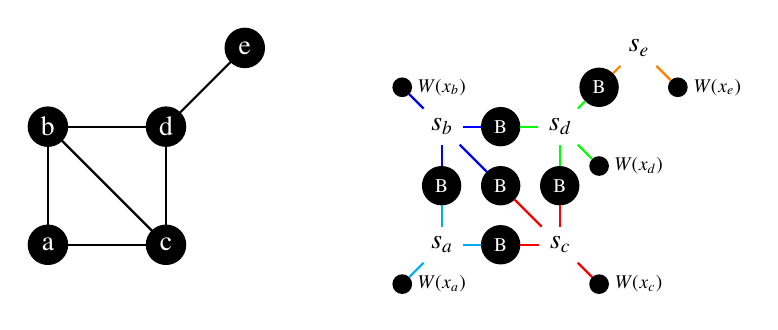
\begin{tikzpicture}[
    dot/.style = {circle, fill, minimum size=#1,
                inner sep=0pt, outer sep=0pt},
    dot/.default = 6pt  % size of the circle diameter 
                    ]  
        \def\dx{0};
        \def\r{0.25cm}
        \filldraw[fill=black] (\dx,0) circle [radius=\r];
        \filldraw[fill=black] (\dx,1.5) circle [radius=\r];
        \filldraw[fill=black] (1.5+\dx,0) circle [radius=\r];
        \filldraw[fill=black] (1.5+\dx,1.5) circle [radius=\r];
        \filldraw[fill=black] (2.5+\dx,2.5) circle [radius=\r];
        \draw [black,thick] (\dx,0) -- (\dx,1.5);
        \draw [black,thick] (\dx,0) -- (1.5+\dx,0);
        \draw [black,thick] (\dx,1.5) -- (1.5+\dx,1.5);
        \draw [black,thick] (1.5+\dx,0) -- (1.5+\dx,1.5);
        \draw [black,thick] (1.5+\dx,0) -- (\dx,1.5);
        \draw [black,thick] (2.5+\dx,2.5) -- (1.5+\dx,1.5);
        \node[color=white] at (\dx,0) {a};
        \node[color=white] at (\dx,1.5) {b};
        \node[color=white] at (1.5+\dx,0) {c};
        \node[color=white] at (1.5+\dx,1.5) {d};
        \node[color=white] at (2.5+\dx,2.5) {e};
        \def\dx{5};
        \def\r{0.25cm}
        \foreach \x/\y/\e in {0.75/0/ac, 0/0.75/ab, 1.5/0.75/cd, 0.75/1.5/bd, 0.75/0.75/bc, 2/2/de}
            \node[color=white,fill=black,dot=2*\r] at (\x+\dx,\y) (\e) {\scriptsize B};
        \foreach \x/\y/\v in {0/0/a, 0/1.5/b, 1.5/0/c, 1.5/1.5/d, 2.5/2.5/e}
            \node[color=black] at (\x+\dx,\y) (\v) {$s_\v$};
        \foreach \x/\y/\v in {-0.5/-0.5/a, -0.5/2.0/b, 2.0/-0.5/c, 2.0/1.0/d, 3.0/2.0/e}
            \node[color=white,fill=black,dot=\r] at (\x+\dx,\y) (\v\v) {};
        \foreach \x/\y/\v in {-0.5/-0.5/a, -0.5/2.0/b, 2.0/-0.5/c, 2.0/1.0/d, 3.0/2.0/e}
            \node[color=black] at (\x+\dx+0.5,\y) {\scriptsize $W(x_\v)$};
        \draw [cyan,thick] (a) -- (aa);
        \draw [cyan,thick] (a) -- (ab);
        \draw [cyan,thick] (a) -- (ac);
        \draw [blue,thick] (b) -- (bb);
        \draw [blue,thick] (b) -- (ab);
        \draw [blue,thick] (b) -- (bc);
        \draw [blue,thick] (b) -- (bd);
        \draw [red,thick] (c) -- (cc);
        \draw [red,thick] (c) -- (ac);
        \draw [red,thick] (c) -- (bc);
        \draw [red,thick] (c) -- (cd);
        \draw [green,thick] (d) -- (dd);
        \draw [green,thick] (d) -- (bd);
        \draw [green,thick] (d) -- (de);
        \draw [green,thick] (d) -- (cd);
        \draw [orange,thick] (e) -- (ee);
        \draw [orange,thick] (e) -- (de);
    \end{tikzpicture}}
    
    The contraction of this tensor network can be done in a pairwise order:
    \begin{align*}
        &\sum_{s_a,s_b,s_c,s_d,s_e} W(x_a)_{s_a} W(x_b)_{s_b} W(x_c)_{s_c} W(x_d)_{s_d} W(x_e)_{s_e} B_{s_a s_b} B_{s_b s_d} B_{s_c s_d} B_{s_a s_c} B_{s_b s_c} B_{s_d s_e}\\
        =&\sum_{s_b,s_c}\left(\sum_{s_d}\left(\left(\left(\left(\sum_{s_e}B_{s_d s_e}W(x_e)_{s_e}\right) W(x_d)_{s_d}\right) \left(B_{s_bs_d} W(x_b)_{s_b}\right)\right) \left(B_{s_cs_d} W(x_c)_{s_c}\right)\right)\right.\\
        &\phantom{XXX}\left.\left(B_{s_bs_c}\left(\sum_{s_a}B_{s_as_b}\left(B_{s_as_c}W(x_a)_{s_a}\right)\right)\right)\right)\\
        =&1 + x_a + x_b + x_c + x_d + x_e + x_ax_d + x_ax_e + x_cx_e + x_bx_e\\
        =&1+5x+4x^2 \qquad \quad (x_{i} = x)
    \end{align*}
\end{example}

Before contracting the tensor network and evaluating the independence polynomial numerically, let us first elevate the tensor elements $0$s and $1$s in tensors $W(x)$ and $B$ from integers and floating point numbers to the additive identity,
$\mymathbb{0}$, and multiplicative identity, $\mymathbb{1}$, of a commutative semiring as discussed in Sec.~\ref{sec:generic}.
The most natural approach is to treat the tensor elements as polynomials and evaluate the polynomial directly.
Let us create a polynomial type, and represent a polynomial $a_0 + a_1 x + \ldots + a_k x^k$ as a coefficient vector $(a_0, a_1, \ldots, a_k) \in \mathbb{R}^k$, so, e.g., $x$ is represented as $(0, 1)$.
We define the algebra between the polynomials $a$ of order $k_a$ and $b$ of order $k_b$ as
\begin{equation}
    \begin{split}
    a \oplus b &= (a_0 + b_0, a_1 + b_1, \ldots, a_{\max(k_a, k_b)} + b_{\max(k_a, k_b)}),\\
    a \odot b &= (a_0 + b_0, a_1b_0 + a_0b_1, a_{2}b_{0} + a_{1}b_{1} + a_{0}b_{2},  \ldots, a_{k_a} b_{k_b}),\\
    \mymathbb{0} &= (),  \\
    \mymathbb{1} &= (1).\label{eq:polynomial}
    \end{split}
\end{equation}
We can see these operations are standard addition and multiplication operations of polynomials, and the polynomial type forms a commutative ring. The tensors $W$ and $B$ can thus be written as 
\begin{equation}
    W^{\rm poly} = \left(\begin{matrix}
        \mymathbb{1} \\
        (0,1)
    \end{matrix}\right),   
    \qquad \qquad
        B^{\rm poly} = \left(\begin{matrix}
        \mymathbb{1}  & \mymathbb{1} \\
        \mymathbb{1} & \mymathbb{0}
    \end{matrix}\right).
\end{equation}
By contracting the tensor network with the polynomial type, the final result is the exact representation of the independence polynomial.
One way to efficiently evaluate the multiplication operation is to use the convolution theorem~\cite{Schonhage1971}, but this approach suffers from a space overhead proportional to $\alpha(G)$ because each polynomial requires a vector of such size to store the coefficients. 

Here, we propose to find the independence polynomial by fitting $\alpha(G)+1$ random values of $x_{i}$ and $y_{i} = I(G,x_{i})$. One can then compute the independence polynomial coefficients $a_{i}$ by solving the linear equation: 
\begin{equation}
\left(\begin{matrix}
1 & x_0 & x_0^2 & \ldots & x_0^{\alpha(G)} \\
1 & x_1 & x_1^2 & \ldots & x_1^{\alpha(G)} \\
\vdots & \vdots & \vdots &\ddots & \vdots \\
1 & x_{\alpha(G)} & x_{\alpha(G)}^2 & \ldots & x_{\alpha(G)}^{\alpha(G)}
\end{matrix}\right)
\left(\begin{matrix}
a_0 \\ a_1 \\ \vdots \\ a_{\alpha(G)}
\end{matrix}\right)
= \left(\begin{matrix}
y_0 \\ y_1 \\ \vdots \\ y_{\alpha(G)}
\end{matrix}\right).\label{eq:lineareq}
\end{equation}
With this approach, we do not incur the linear overhead in space. However, because the independence polynomial coefficients can have a huge order-of-magnitude range, if we use floating point numbers in the computation, the round-off errors can be significant for the counting of large independent set sizes.
In addition, the number could easily overflow if we use fixed-width integer types.
The big integer type is also not a good option because big integers with varying width can be very slow and is incompatible with graphics processing unit (GPU) devices. These problems can be solved by introducing a finite-field algebra $\text{GF}(p)$:
\begin{equation}
\begin{split}
    x ~\oplus~ y &= x+y\pmod p,\\
    x ~\odot~ y &= xy\pmod p,\\
    \mymathbb{0} &= 0,\\
    \mymathbb{1} &= 1.
\end{split}\label{eq:finitefield}
\end{equation}
With a finite-field algebra, we have the following observations:
\begin{enumerate}
    \item One can use Gaussian elimination~\cite{Golub2013} to solve the linear equation \Eq{eq:lineareq} since it is a generic algorithm that works for any elements with field algebra. The multiplicative inverse of a finite-field algebra can be computed with the extended Euclidean algorithm.
    \item Given the remainders of a larger unknown integer $x$ over a set of co-prime integers $\{p_1, p_2, \ldots, p_n\}$,
    $x \pmod {p_1 \times p_2 \times \ldots \times p_n}$ can be computed using the Chinese remainder theorem. With this, one can infer big integers from small integers.
\end{enumerate}
With these observations, we develop Algorithm~\ref{alg:finitefield} to compute the independence polynomial exactly without introducing space overheads.
This is an iterative algorithm that tries different prime numbers $p$ until convergence.
In each iteration, we contract the tensor networks to evaluate the polynomial for each $x_{i}$ on the finite field algebra ${\rm GF}(p)$.
Let use denote the results as $Y$, then we solve a linear equation $Y = X A_p$ using the gaussian elimination on ${\rm GF}(p)$ to find the coefficient modulo $p$, $A_p \equiv A \pmod p$.
Finally we apply the Chinese remainder theorem to get $A \pmod {P\times p}$, where $P$ is a product of all prime numbers chosen in previous iterations.
If this number does not change compared with the previous iteration, it indicates the result has converged.
All computations are done with integers of fixed width $W$ except the last step of applying the Chinese remainder theorem.
In \App{app:fft}, we provide another method to solve the linear equation using discrete Fourier transform.

\LinesNumberedHidden
\begin{algorithm}[!ht]
    \small
    \SetAlgoNoLine
    %\LinesNumbered
    Let $P = 1$, $W$ be the integer width, vector $\chi = (0,1,2, \ldots, \alpha(G))$, matrix $X_{ij} = (\chi_i)^j$, where $i,j = 0, 1, \ldots, \alpha(G)$\;

    \While{true}{
        compute the largest prime $p$ that $\gcd(p, P) = 1$ and $p \leq 2^W$\;

        \For{$i=1\ldots\alpha(G)$}{
            t = ${\rm tensor\_network}(\chi_i\pmod p)$ \tcp*[l]{defined on $\text{GF}(p)$}

            $Y_i \pmod p  = {\rm contract}(t)$\;
        }

        $A_p = (a_0, a_1, \ldots, a_{\alpha(G)}) \pmod p = {\rm gaussian\_elimination}(X, Y \pmod p) $\;

        $A_{P\times p} = {\rm chinese\_remainder}(A_P, A_p)$\;

        \If{$A_P = A_{P \times p}$}{
            \Return $A_P$ \tcp*[l]{converged}
        }
        $P = P \times p$\;
    }\caption{Compute the independence polynomial exactly without integer overflow}\label{alg:finitefield} 
\end{algorithm}

\subsection{Maximal independence polynomial}
Sometimes, one may be interested in knowing maximal solutions to understand why his or her programs are trapped in a local minimum.
In this paper, the term ``maximal'' has a different meaning from ``maximum''  which we discussed in the previous sections; a maximal independent set is an independent set that is not a subset of any other independent set, but its size may not be the maximum.
Instead of counting all independent sets, the maximal independence polynomial counts the number of maximal independent sets of various sizes~\cite{Hu2017}.
 Concretely, it is defined as
\begin{equation}
I_{\rm max}(G, x) = \sum_{k=0}^{\alpha(G)} b_k x^k,
\end{equation}
where $b_k$ is the number of maximal independent sets of size $k$ in $G$.
Obviously, $b_{k} \leq a_{k}$ and $b_{\alpha(G)} = a_{\alpha(G)}$. $I_{\rm max}(G, 1)$ counts the total number of maximal independent sets~\cite{Gaspers2012, Manne2013}, where the fastest algorithm currently has a runtime of $O(1.3642^{|V|})$~\cite{Gaspers2012}.
If we want to find an MIS, $b_{k}$ counts the number of local optimum at size $k < \alpha(G)$, and can, in some cases, provide hints on the difficulty of finding the MIS using local algorithms~\red{cite experiment}.
The uni-modality, log-concavity, and real-rootness properties of the maximal independence polynomial for special classes of graphs have also been studied~\cite{Hu2017}. 

Let us denote the neighborhood of a vertex $v$ as $N(v)$ and denote $N[v] = N(v)\cup \{v\}$.
A maximal independent set $I_m$ is an independent set where there exists no vertex $v$ such that $I_m \cap N[v]  = \emptyset$.
We can modify the tensor network for computing the independence polynomial to include this restriction. Instead of defining the restriction on vertices and edges, it is more natural to define it on $N[v]$:
\begin{equation}\label{eq:maximal}
    T(x_v)_{s_1,s_2,\ldots,s_{|N(v)|},s_v} = \begin{cases}
        s_vx_v & s_1=s_2=\ldots=s_{|N(v)|}=0,\\
        1-s_v& \text{otherwise}.\\
    \end{cases}
\end{equation}
Intuitively, it means if all the neighborhood vertices are not in $I_{m}$, i.e., $ s_1=s_2=\ldots=s_{|N(v)|}=0$, then $v$ should be in $I_{m}$, counted as $x_{v}$,
and if any of the neighborhood vertices is in $I_{m}$, i.e., $\exists i \in \{1,2,\ldots, |N(v)|\}$ s.t. $s_{i} = 1$, then $v$ cannot be in $I_{m}$.
As an example, for a vertex of degree 2, the resulting rank-3 tensor is
\begin{equation}
    T(x_v)=\left(\begin{matrix}
    \left(\begin{matrix}
        0 &1 \\
        1 &1
    \end{matrix}\right)\\
    \left(\begin{matrix}
        x_v &0 \\
        0 &0
    \end{matrix}\right)
    \end{matrix}\right).
\end{equation}
 
With the tensors defined as $T(x_v)$, we can perform a similar computation of contracting the tensor network with the same tensor element types as described in the previous section~\ref{sec:indpoly}, the result of which then produces the maximal independence polynomial. Let us consider the example in~\Sec{eg:tensorcontraction}: its corresponding tensor network structure for computing the maximal independent polynomial becomes

    \centerline{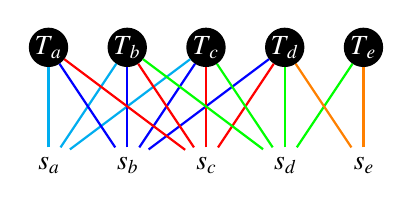
\begin{tikzpicture}[
    dot/.style = {circle, fill, minimum size=#1,
                inner sep=0pt, outer sep=0pt},
    dot/.default = 6pt  % size of the circle diameter 
                    ]  
        \def\dx{0};
        \def\r{0.5cm}
        \def\G{1.0}
        \foreach \x/\y/\v in {0/0/a, 1/0/b, 2/0/c, 3/0/d, 4/0/e}
            \node[color=black] at (\x*\G+\dx,\y) (\v) {$s_\v$};
        \foreach \x/\v/\t in {0/A/$T_a$, 1/B/$T_b$, 2/C/$T_c$, 3/D/$T_d$, 4/E/$T_e$}
            \node[color=white,fill=black,dot=\r] at (\x*\G+\dx,1.5) (\v) {\t};
        \draw [cyan,thick] (a) -- (A);
        \draw [cyan,thick] (a) -- (B);
        \draw [cyan,thick] (a) -- (C);
        \draw [blue,thick] (b) -- (B);
        \draw [blue,thick] (b) -- (A);
        \draw [blue,thick] (b) -- (C);
        \draw [blue,thick] (b) -- (D);
        \draw [red,thick] (c) -- (C);
        \draw [red,thick] (c) -- (A);
        \draw [red,thick] (c) -- (B);
        \draw [red,thick] (c) -- (D);
        \draw [green,thick] (d) -- (D);
        \draw [green,thick] (d) -- (B);
        \draw [green,thick] (d) -- (C);
        \draw [green,thick] (d) -- (E);
        \draw [orange,thick] (e) -- (E);
        \draw [orange,thick] (e) -- (D);
    \end{tikzpicture}}
 
One can see that the average degree of a tensor is increased.
The computational complexity of this new tensor network contraction is often greater than the one for computing the independence polynomial.
However, in most sparse graphs, this tensor network contraction approach is still significantly faster than enumerating all the maximal cliques on its complement graph using the Bron-Kerbosch algorithm~\cite{Bron1973}, which is the standard algorithm that we are aware of to compute the maximal independence polynomial.

\section{Maximum independent sets and its counting problem}
\subsection{Tropical algebra for finding the independence number and counting MISs}
In the previous section, we focused on computing the independence polynomial for a graph $G$ of given independence number $\alpha(G)$, but we did not show how to compute this number.
The method we use to compute this quantity is based on the following observations. Let $x=\infty$, the independence polynomial becomes
\begin{equation}
I(G, \infty) = a_{\alpha(G)} \infty^{\alpha(G)},
\end{equation}
where the lower-order terms vanish. We can thus replace the polynomial type $a = (a_0, a_1, \ldots, a_k)$ with $a(k) = (a_{k}, k)$, where the second element stores the largest exponent $k$ and the first element stores the corresponding coefficient $a_{k}$.
From this, we can define a new algebra as \red{I've changed this, but I don't have strong feelings about this. We can certainly consider changing back.
I thought this would be more consistent with the earlier notations and show how it's stored in the program as well.}
\blue{I prefer the previous one, what about you @XG?}
\begin{equation}
\begin{split}
    a(k) \oplus a(j) &= \begin{cases}
        \left(a_k + a_j, \max(k,j) \right), & k = j \\
        \left(a_j, \max(k,j) \right), & k < j \\
        \left(a_k, \max(k,j) \right), & k > j
    \end{cases}, \\
    a(k) \odot a(j) &= (a_k a_j, k+j) \\
    \mymathbb{0} &= (0, -\infty)\\
    \mymathbb{1} &= (1, 0). \label{eq:countingtropical}
\end{split}
\end{equation}
%\begin{equation}
%\begin{split}
%    a_x\infty^x \oplus a_y\infty^y &= \begin{cases}
%        (a_x + a_y)\infty^{\max(x,y)}, & x = y\\
%        a_y\infty^{\max(x,y)}, & x < y\\
%        a_x\infty^{\max(x,y)}, & x > y
%    \end{cases}, \\
%    a_x\infty^x \odot a_y\infty^y &= a_x a_y\infty^{x+y}\\
%    \mymathbb{0} &= 0\infty^{-\infty}\\
%    \mymathbb{1} &= 1\infty^{0}. \label{eq:countingtropical}
%\end{split}
%\end{equation}
% In the program, we only need to store the exponent $x$ and the corresponding coefficient $a_x$ initialized to $1$. 
The algebra of the exponents becomes the max-plus tropical algebra: $k \oplus j = \max(k,j)$ and $k \odot j = k + j$~\cite{Maclagan2015, Moore2011}.
This algebra is the same as the one used in Liu et al.~\cite{Liu2021} to calculate and count spin glass ground states.
For independent set calculations here, the vertex tensor and edge tensor becomes:
\begin{equation}
    W^{\rm tropical} = \left(\begin{matrix}
        \mymathbb{1} \\
        (1,1)
    \end{matrix}\right),   
    \qquad \qquad
        B^{\rm tropical} = \left(\begin{matrix}
        \mymathbb{1}  & \mymathbb{1} \\
        \mymathbb{1} & \mymathbb{0}
    \end{matrix}\right).
\end{equation}

\subsection{Truncated polynomial algebra for counting independent sets of large size}
Instead of counting just the MISs, one may be interested in counting the independent sets of large sizes close to the MIS size.
For example, if one is interested in counting only $a_{\alpha(G)}$ and $a_{\alpha(G)-1}$, we can define a truncated polynomial algebra by keeping only the largest two coefficients in the polynomial in \Eq{eq:polynomial}:
\begin{equation}
    \begin{split}
    a \oplus b &= (a_{\max(k_a, k_b)-1} + b_{\max(k_a, k_b)-1}, a_{\max(k_a, k_b)} + b_{\max(k_a, k_b)}),\\
    a \odot b &= (a_{k_a-1} b_{k_b}+a_{k_a} b_{k_b-1}, a_{k_a} b_{k_b}),\\
    \mymathbb{0} &= (), \\
    \mymathbb{1} &= (1).\label{eq:max2poly}
    \end{split}
\end{equation}
In the program, we thus need a data structure that contains three fields, the largest order $k$, and the coefficients for the two largest orders $a_k$ and $a_{k-1}$.
This approach can clearly be extended to calculate more independence polynomial coefficients and is more efficient than calculating the entire independence polynomial.
As will be shown below, this algebra can also be extended to enumerate those large-size independent sets.

\section{Enumeration of configurations and enumeration bounds}
\subsection{Enumeration of MIS configurations}
The enumeration problems of independent sets are also interesting and has been studied extensively in the literature~\cite{Bron1973, Eppstein2010, Johnson1988}, including,
for example, the enumeration of all independent sets, the enumeration of all maximal independent sets, or the enumeration of all MISs.
The standard algorithm to enumerate all maximal independent sets is the Bron-Kerbosch algorithm~\cite{Bron1973}, which, of course, includes the enumeration of all MISs and can be used to enumerate all independent sets as well.
Here, we adapt the tensor element types for different enumeration problems.
For example, our tensor-network based algorithm to enumerate all MISs is expectedly much faster and more space-efficient than the Bron-Kerbosch algorithm, which lists all maximal independent sets. 

To enumerate all independent sets, we input a set of configurations into the tensor elements. More concretely, we design a new element type having the following algebra
\begin{equation}
\begin{split}
    s \oplus t &= s \cup t\\
    s \odot t &= \{\sigma \lor^\circ \tau \, | \, \sigma \in s, \tau \in t\}\\
    \mymathbb{0} &= \{\}\\
    \mymathbb{1} &= \{0^{\otimes |V|}\}.
\end{split}\label{eq:set}
\end{equation}
where $s$ and $t$ are each a set of $|V|$-bit strings and $\lor^\circ$ is the bitwise OR operation over two bit strings.
\begin{example}\label{eg:setalgebra}
    For elements being bit vectors of length $5$, we have the following set algebra
\begin{equation*}
\begin{split}
    &\{00001\} \oplus \{01110, 01000\} = \{01110, 01000\} \oplus \{00001\} = \{00001,01110, 01000\}\\
    &\{00001\} \oplus \{\} = \{\}\\
&\\
    &\{00001\} \odot \{01110, 01000\} = \{01110, 01000\} \odot \{00001\} = \{01111, 01001\}\\
    &\{00001\} \odot \{\} = \{\}\\
    &\{00001\} \odot \{00000\} = \{00001\}
\end{split}
\end{equation*}
\end{example}

The variable $x_{i}$ in the vertex tensor is initialized to $x_i = \{\boldsymbol{e}_{i}\}$, where $\boldsymbol{e}_i$ is the standard basis vector of size $|V|$ and having 1 at index $i$. The vertex and edge tensors are thus
\begin{equation}
    W^{\rm enum}(\{\boldsymbol{e}_{i}\}) = \left(\begin{matrix}
        \mymathbb{1} \\
        \{\boldsymbol{e}_{i}\}
    \end{matrix}\right),   
    \qquad \qquad
        B^{\rm enum} = \left(\begin{matrix}
        \mymathbb{1}  & \mymathbb{1} \\
        \mymathbb{1} & \mymathbb{0}
    \end{matrix}\right).
\end{equation}

This set algebra can serve as the first element in \Eq{eq:countingtropical} to enumerate all MISs, \Eq{eq:polynomial} to enumerate independent sets of different sizes,
or \Eq{eq:max2poly} to enumerate all independent sets of size $\alpha(G)$ and $\alpha(G)-1$.
For example, to enumerate only the MISs, with the tropical algebra, we define $s(k) = (s_{k}, k)$, where the first element follows the algebra in \Eq{eq:set} and the second element follows the max-plus tropical algebra.
The combined operations become: 
\begin{equation}
\begin{split}
    s(k) \oplus s(j) &= \begin{cases}
        \left(s_k \cup s_j, \max(k,j) \right), & k = j \\
        \left(s_j, \max(k,j) \right), & k < j \\
        \left(s_k, \max(k,j) \right), & k > j
    \end{cases}, \\
    s(k) \odot s(j) &= (\{\sigma \lor^\circ \tau \, | \, \sigma \in s_k, \tau \in s_j\}, k+j) \\
    \mymathbb{0} &= (\{ \}, -\infty)\\
    \mymathbb{1} &= (\{0^{\otimes |V|}\}, 0). \label{eq:countingtropicalset}
\end{split}
\end{equation}
%\begin{equation}
%\begin{split}
%    s_x\infty^x \oplus s_y\infty^y &= \begin{cases}
%        (s_x \cup s_y)\infty^{\max(x,y)}, & x = y\\
%        s_y\infty^{\max(x,y)}, & x < y\\
%        s_x\infty^{\max(x,y)}, & x > y
%    \end{cases},\\
%    s_x\infty^x \odot s_y\infty^y &= \{\sigma \lor^\circ \tau | \sigma \in s_x, \tau \in s_y\}\infty^{x+y},\\
%    \mymathbb{0} &= \{\}\infty^{-\infty},\\
%    \mymathbb{1} &= \{0^{\otimes |V|}\}\infty^{0},
%\end{split}
%\end{equation}
Clearly, the vertex tensor and edge tensor become
\begin{equation}
    W^{\rm MISenum}(\{\boldsymbol{e}_{i}\}) = \left(\begin{matrix}
        \mymathbb{1} \\
        \left({\{\boldsymbol{e}_{i}\}, 1} \right)
    \end{matrix}\right),   
    \qquad \qquad
        B^{\rm MISenum} = \left(\begin{matrix}
        \mymathbb{1}  & \mymathbb{1} \\
        \mymathbb{1} & \mymathbb{0}
    \end{matrix}\right).
\end{equation}
The contraction of the corresponding tensor network yields an enumeration of all MIS configurations.

If one is interested in obtaining only a single MIS configuration, one can just keep a single configuration in the intermediate computations to save the computational effort.
Here is a new algebra defined on the bit strings, replacing the sets of bit strings in \Eq{eq:set}, 
%We leave this as an exercise for readers.
%
%\iffalse
%\begin{equation}
%\begin{split}
%    \sigma_x\infty^x \oplus \sigma_y\infty^y &= \begin{cases}
%        {\rm select}(\sigma_x, \sigma_y)\infty^{\max(x,y)}, & x = y\\
%        \sigma_y\infty^{\max(x,y)}, & x < y\\
%        \sigma_x\infty^{\max(x,y)}, & x > y
%    \end{cases},\\
%    \sigma_x\infty^x \odot \sigma_y\infty^y &= (\sigma_x \lor^\circ \sigma_y)\infty^{x+y},\\
%    \mymathbb{0} &= 1^{\otimes n}\infty^{-\infty},\\
%    \mymathbb{1} &= 0^{\otimes n}\infty^{0},
%\end{split}
%\end{equation}
%\fi
\begin{equation}
\begin{split}
    \sigma \oplus \tau &= {\rm select}(\sigma, \tau), \\
    \sigma \odot \tau &= (\sigma\lor^\circ \tau),\\
    \mymathbb{0} &= 1^{\otimes |V|}, \\
    \mymathbb{1} &= 0^{\otimes |V|},
\end{split}\label{eq:singleconfig}
\end{equation}
where the \texttt{select} function picks one of $\sigma$ and $\tau$ by some criteria to make the algebra commutative and associative, e.g. by picking one with a smaller integer value.
%In practice, we can just pick randomly from them, in which case the program will output one of the MIS configurations randomly.

% Although the above discussion is in the context of the MIS problem, we can also combine the above algebras with the maximal independence network in \Eq{eq:maximal} to enumerate or sample maximal independent sets,
% as well as other problems in \App{app:otherproblems} for configuration enumeration and sampling.

\subsection{Bounding the MIS enumeration space}
When we use the algebra in \Eq{eq:countingtropicalset} to enumerate all MIS configurations, we find that the program stores significantly more intermediate configurations than necessary and thus incur significant overheads in space.
To speed up the computation and reduce space overhead, we use $\alpha(G)$ to bound the searching space.
First, we compute the value of $\alpha(G)$ with tropical algebra and cache all intermediate tensors.
Then, we compute a boolean mask for each cached tensor, where we use a boolean true to represent a tensor element having a contribution to the MIS (i.e.\ with a non-zero gradient) and boolean false otherwise.
Finally, we perform masked matrix multiplication using the new element type with the above algebra, \Eq{eq:countingtropicalset}, for obtaining all configurations.
Note that these masks in fact correspond to tensor elements with non-zero gradients with respect to the MIS size; we compute these masks by back propagation of the gradients.
To derive the back-propagation rule for tensor contraction,
we first reduce the problem to finding the back-propagation rule of a tropical matrix multiplication $C = A B$.
Since $ C_{ik} = \bigoplus_{j} \ A_{ij} \odot B_{jk} = \max_{j} \ A_{ij} \odot B_{jk}$ with tropical algebra, we have the following inequality
\begin{equation}
    A_{ij} \odot B_{jk} \leq C_{ik}.
\end{equation}
Here $\leq$ on tropical numbers are the same as the real-number algebra.
The equality holds for some $j'$, which means $A_{ij'}$ and $B_{j'k}$ have contributions to $C_{ik}$.
Since $A_{ij} \odot B_{jk} = A_{ij} + B_{jk}$, one can move $B_{jk}$ to the right hand side of the inequality: 
\begin{equation}
    A_{ij} \leq C_{ik} \odot B_{jk}^{\circ -1}
\end{equation}
where ${}^{\circ -1}$ is the element-wise multiplicative inverse on tropical algebra (which is the additive inverse on real numbers).
The inequality still holds if we take the minimum over $k$: 
\begin{equation}
    A_{ij} \leq \min_{k}(C_{ik} \odot B_{jk}^{\circ -1}) = \left(\max_{k} \left(C_{ik}^{\circ -1} \odot B_{jk} \right) \right)^{\circ -1} = \left(\bigoplus_{k} \left(C_{ik}^{\circ -1} \odot B_{jk} \right) \right)^{\circ -1} = \left( C^{\circ-1} B^{\mathsf{T}} \right)^{\circ -1}_{ij}.
\end{equation}
On the right hand side, we transform the operation into a tropical matrix multiplication so that we can utilize the fast tropical BLAS routines~\cite{TropicalGEMM}.
Again, the equality holds if and only if the element $A_{ij}$ has a contribution to $C$ (i.e.\ having a non-zero gradient).
Let the gradient mask for $C$ be $\overline C$; the back-propagation rule for gradient masks reads
\begin{equation}
\overline{A}_{ij} = \delta \left(A_{ij}, \left( \left( C^{\circ-1} \circ \overline C \right) B^{\mathsf{T}} \right)_{ij}^{\circ -1} \right),
\end{equation}
where $\circ$ is the element-wise product, boolean false is treated as the tropical number $\mymathbb{0}$, and boolean true is treated as the tropical number $\mymathbb{1}$.
This rule defined on matrix multiplication can be easily generalized to tensor contraction by replacing the matrix multiplication between $C^{\circ-1} \circ \overline C$ and $B^{\mathsf{T}}$ by a tensor contraction.
With the above method, one can significantly reduce the space needed to store the intermediate configurations.

\section{Benchmarks and case studies}
\subsection{Performance benchmarks}
We run a single thread benchmark on CPU Intel(R) Xeon(R) CPU E5-2686 v4 @ 2.30GHz,
and its CUDA version on a GPU Tesla V100.
The results are shown in Figure~\ref{fig:benchmark}.
The graph we use are random 3 regular graphs, a typical type of sparse graph that having small tree width $\text{tw}(G) \leq |V|/6$~\cite{Fomin2006}.


\begin{figure} 
    \centering
    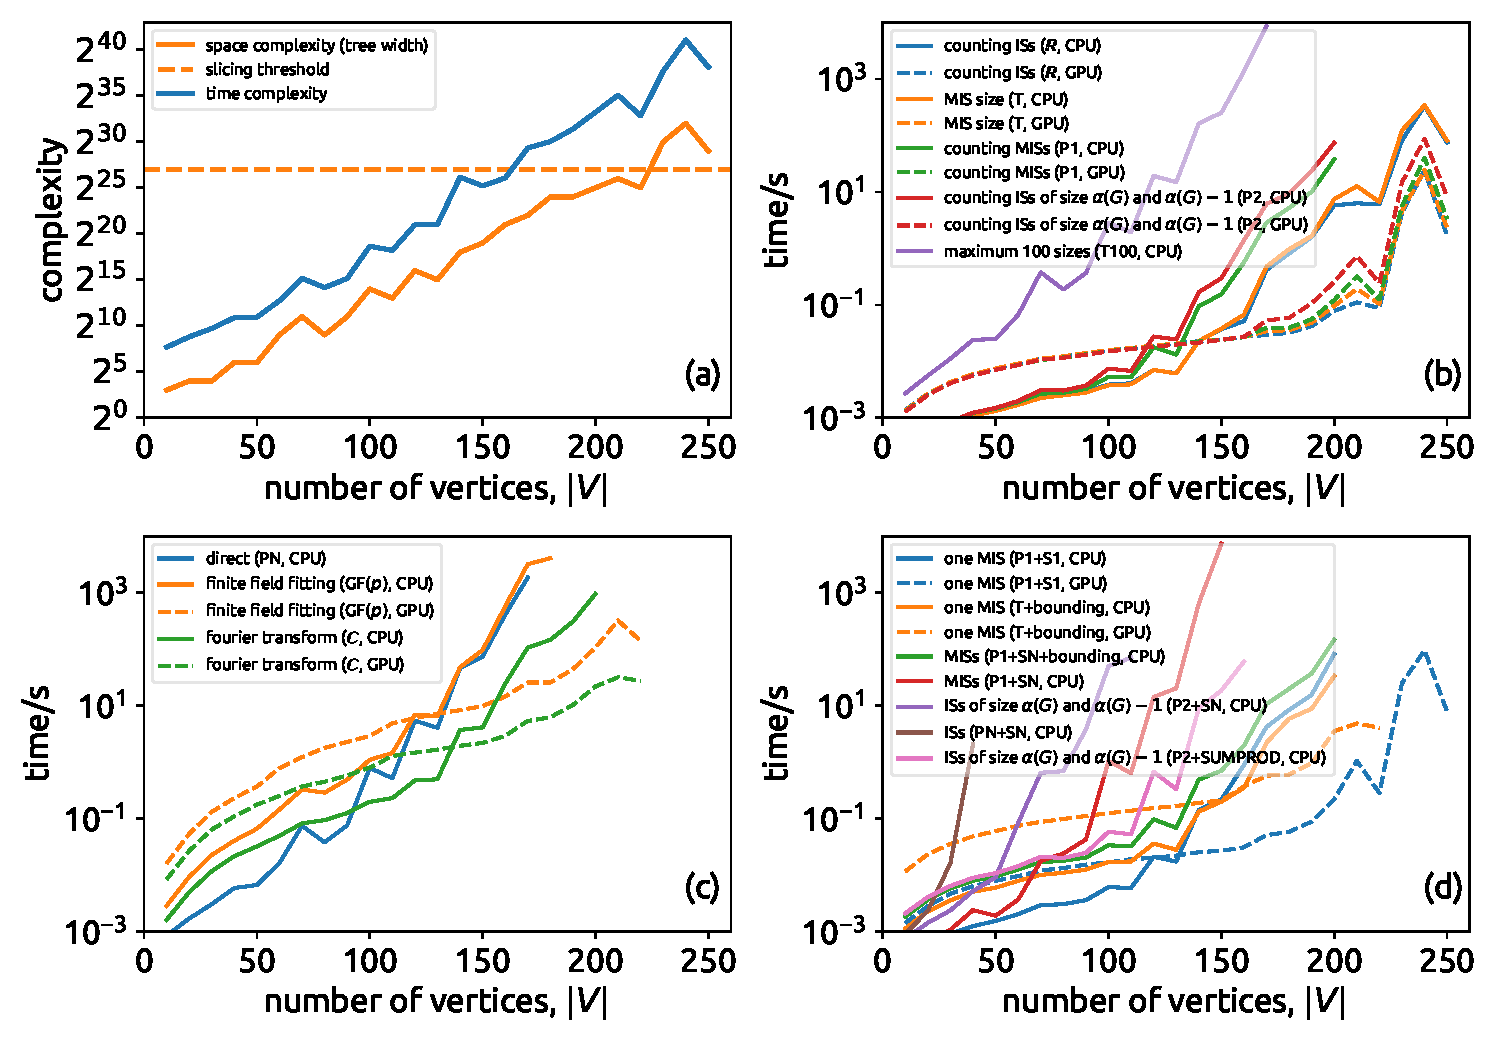
\includegraphics[width=\textwidth, trim={0cm 0cm 0cm 0cm}, clip]{figures/fig1.pdf}
    \caption{Benchmark results for computing different properties of independent sets on a random three regular graph with different tensor element types.
    (b) is the computing time for computing maximum independent set size, number of independent sets and suboptimal sets.
    (c) is the computing time for independence polynomials with different approaches.
    (d) is the computing time for finding all configurations and a single configuration, with or without bounding.
    }
    \label{fig:benchmark}
\end{figure}

Among the benchmarks shown in \Fig{fig:benchmark}, computing \texttt{max size (CPU)},
\texttt{total size (CPU)}, \texttt{total size (GPU)}, \texttt{IDP (FFT) (CPU)}, \texttt{IDP (FFT) (GPU)} and \texttt{single configuration (bounding) (CPU)} can utilize fast BLAS functions,
hence they are relatively faster comparing to other methods in the same category.
Only algebras requiring dynamic sized structures can not be computed on GPU, here are polynomial algebra for computing independence polynomial and set algebra for enumerating configurations.
When computing the independence polynomial, the finite field approach is the only method without round off error that can run on GPU.
To enumerate the MISs, the technique to bound the enumeration space is important,
without which the largest enumeratible size is only $150$ with 32G memory while being one order slower.
All these computing times have strong correlation with the tree width,
while the computing times of configurations enumeration also depends on the size of target configuration space.

\subsection{Example case studies} In this section, we give a few examples where the different properties of independence sets are used.
In all the examples, the types of graphs we used are shown in Figure~\ref{fig:lattices}, where vertices are all placed on square lattices with lattice dimensions $L \times L$.
The graphs include: the square grid graphs, denoted as SG; the square grid graphs with a filling factor $p$, denoted as SG$(p)$, where $\lfloor pL^{2} \rfloor$ square grids are occupied with vertices;
the King's graphs, denoted as K; the King's graphs with a filling factor $p$, denoted as K$(p)$. 

\begin{figure}[t] 
    \centering
    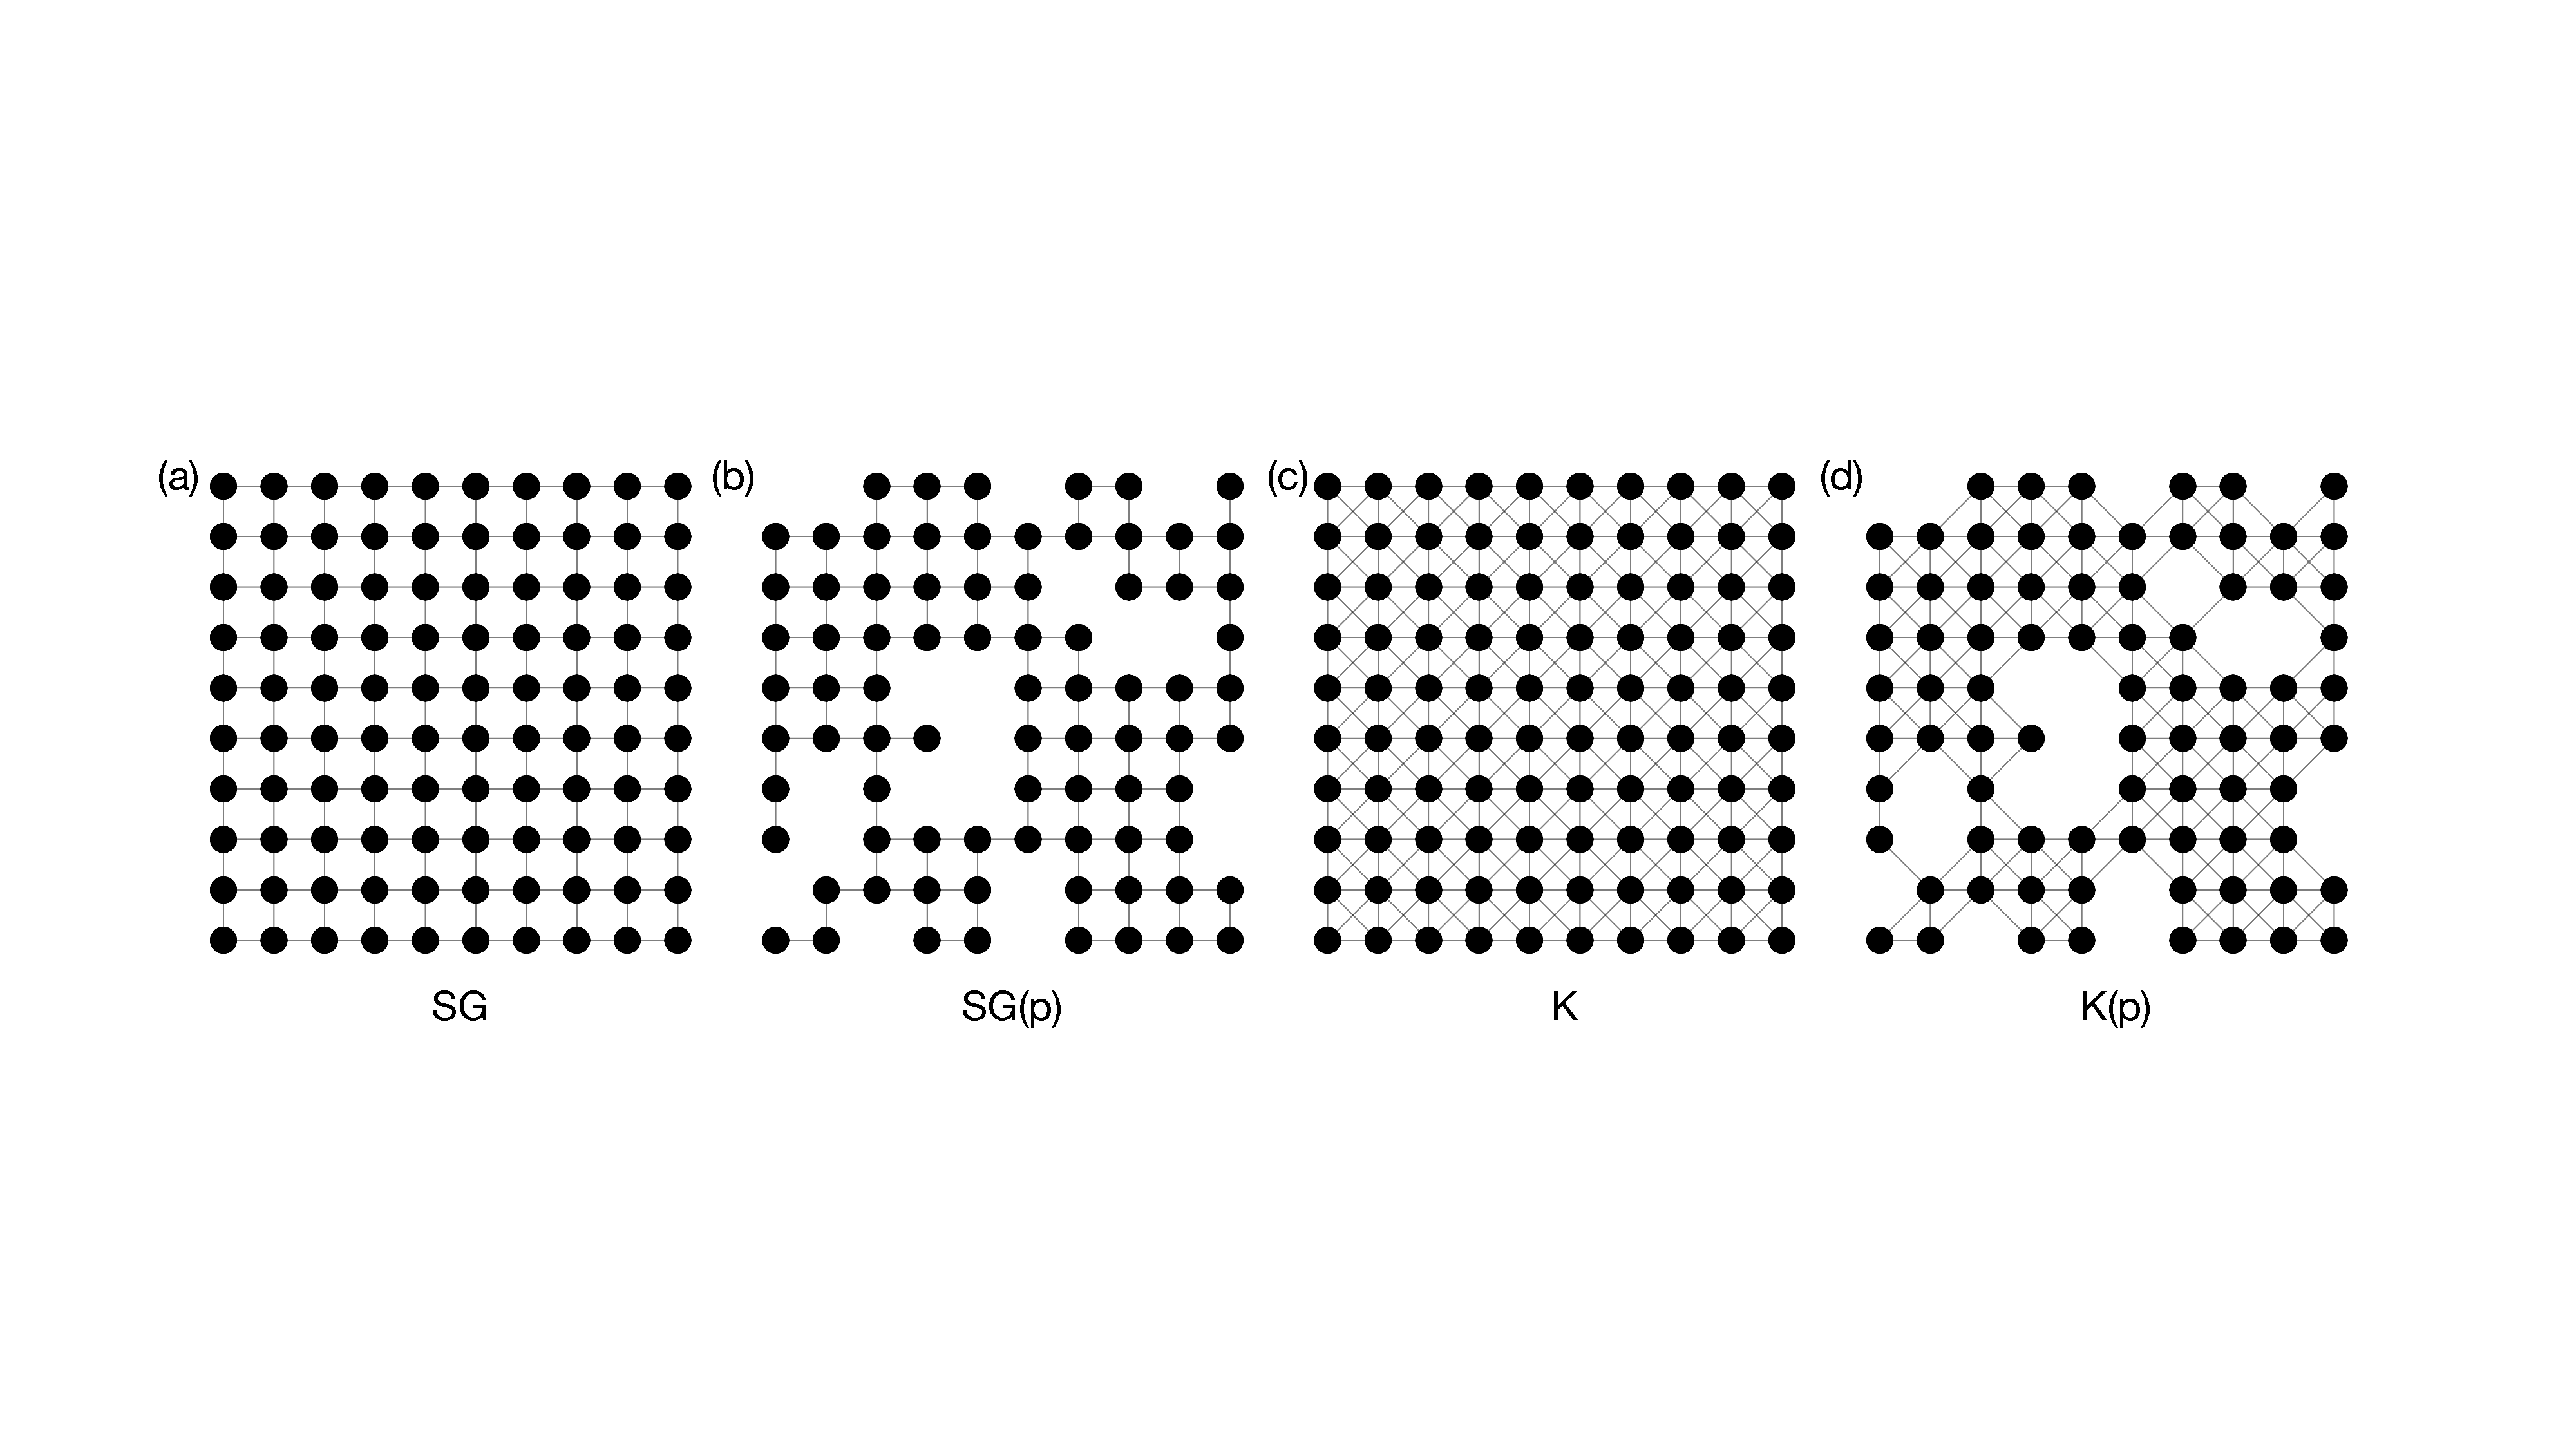
\includegraphics[width=\textwidth, trim={0cm 0cm 0cm 0cm}, clip]{lattices.pdf}
    \caption{The types of graphs used in the benchmark and case studies.
    The lattice dimensions are $L\times L$. (a) Square grid graph denoted as SG. (b) Square grid graph with a filling factor $p=0.8$, denoted as SG(0.8).
    (c) King's graph denoted as K. (d) King's graph with a filling factor $p=0.8$, denoted as K(0.8).}
    \label{fig:lattices}
\end{figure}

\subsubsection{Number of independent sets and hard-square entropy constant}
The number of independent sets for square grid graphs of size $L \times L$ form a well-known integer sequence (\href{https://oeis.org/A006506}{OEIS A006506}), which is thought as a two-dimensional generalization of the Fibonacci numbers.

\subsubsection{Euler characteristics of independence complex}

\subsubsection{Partition functions and finite-temperature phase transitions}



\section{Discussion and conclusion}
We have introduced a new approach based on tensor network contraction to compute the independence number, independence polynomial, maximal independence polynomial, and enumeration of MIS configurations.
We derived the backward rule for tropical tensor network to bound the search of solution space.
Although many of these properties are global, we can encode them to different tensor element types as commutative semirings.
The power of our tensor network approach is not only limited to the independent set problem, in \App{app:otherproblems}, we show how to map the matching problem and $k$-coloring problem to a tensor network.
Here, we want to discuss more from the programming perspective.
We show some of the Julia language~\cite{Bezanson2012} implementations in Appendix~\ref{sec:technical} and you will find it surprisingly short.
What we need to do is just defining two operations $\oplus$ and $\odot$ and two special elements $\mymathbb{0}$ and $\mymathbb{1}$.
The style that we program is called generic programming,
meaning one can feed different data types into the same program, and the program will compute the result with a proper performance.
In C++, one can use templates for such a purpose.
We chose Julia because its just-in-time compiling is very powerful that it can generate fast code dynamically for users.
Elements of fixed size, such as the finite-field algebra, truncated polynomial, tropical number and tropical number with counting or configuration field described in this paper can all be inlined in an array.
Furthermore, these inlined arrays can be uploaded to GPU devices for faster computation with generic matrix multiplication implemented in CUDA.jl~\cite{Besard2018}.

\section*{Acknowledgments}
We would like to thank Pan Zhang for sharing his code for optimizing contraction orders of a tensor network, his code plays a crucial role in our code base.
We would like to acknowledge Sepehr Ebadi, Maddie Cain and Leo Zhou for popping up inspiring questions,
their questions are the driving force of this project.
Thank Chris Elord for helping us writing the fastest matrix multiplication libary for GEMM, TropicalGEMM.jl, he is a remarkable guy!
\blue{funding information}

\bibliographystyle{siamplain}
\bibliography{refs}

\appendix

\section{Technical guide}\label{sec:technical}
\begin{description}
	\item[OMEinsum] a package for the \texttt{einsum} function,
	\item[OMEinsumContractionOrders] a package for finding the optimal contraction order for the \texttt{einsum} function \\ \href{https://github.com/Happy-Diode/OMEinsumContractionOrders.jl}{https://github.com/Happy-Diode/OMEinsumContractionOrders.jl},
	\item[TropicalGEMM] a package for efficient tropical matrix multiplication (compatible with OMEinsum),
	\item[TropicalNumbers] a package providing tropical number types and tropical algebra, one o the dependency of TropicalGEMM,
	\item[LightGraphs] a package providing graph utilities, like random regular graph generator,
	\item[Polynomials] a package providing polynomial algebra and polynomial fitting,
	\item[Mods and Primes] packages providing finite field algebra and prime number generators.
\end{description}

One can install these packages by opening a Julia REPL, type \colorbox{lightgray}{\texttt{]}} to enter the \texttt{pkg>} mode and type, e.g.
\begin{lstlisting}
pkg> add OMEinsum LightGraphs Mods Primes FFTW Polynomials TropicalNumbers
\end{lstlisting}

It may surprise you that the Julia implementation of algorithms introduced in the paper is so short that except the bounding and sparsity related parts,
all are contained in this appendix. After installing required packages, one can open a Julia REPL and copy the following code into it.

\lstinputlisting[breaklines]{../democode/demo.jl}

In the above examples, the configuration enumeration is very slow, one should use the optimal MIS size for bounding as described in the main text.
We will not show any example about implementing the backward rule here because it has approximately 100 lines of code.
Please checkout our GitHub repository \href{https://github.com/Happy-Diode/NoteOnTropicalMIS}{https://github.com/Happy-Diode/NoteOnTropicalMIS}.

\section{Why not introducing \texorpdfstring{$\delta$} tensors}\label{app:tensorbad}

Given a graph

\centerline{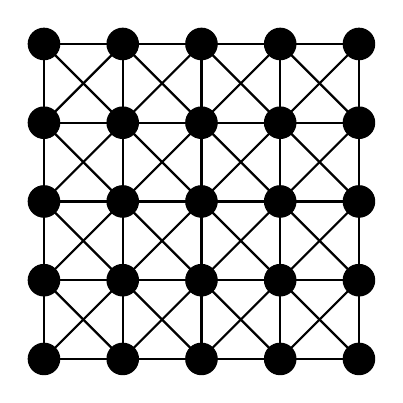
\begin{tikzpicture}
    \def\r{0.2}
    \foreach \x in {1,...,5}
        \foreach \y in {1,...,5}
            \filldraw[fill=black] (\x,\y) circle [radius=\r];
    \foreach \x in {1,...,5}
        \foreach \y in {1,...,4}{
            \draw [black,thick] (\x,\y) -- (\x,\y+1);
            \draw [black,thick] (\y,\x) -- (\y+1,\x);
        }
    \foreach \x in {1,...,4}
        \foreach \y in {1,...,4}{
            \draw [black,thick] (\x,\y) -- (\x+1,\y+1);
            \draw [black,thick] (\y+1,\x) -- (\y,\x+1);
        }
\end{tikzpicture}}

Its traditional tensor network representation with $\delta$ tensors is

\centerline{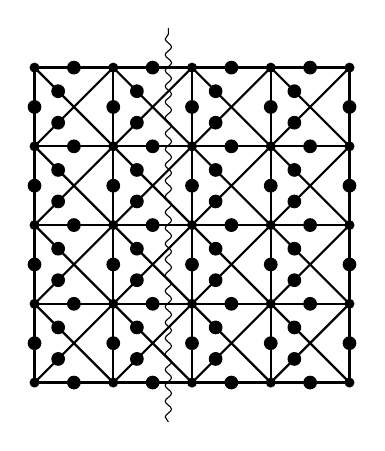
\begin{tikzpicture}
    \def\r{0.08}
    \def\a{0.1}
    \foreach \x in {1,...,5}
        \foreach \y in {1,...,5}
            \filldraw[fill=black] (\x,\y) circle [radius=0.7*\r];
    \foreach \x in {1,...,5}
        \foreach \y in {1,...,4}{
            \filldraw[fill=black] (\x,\y+0.5) circle [radius=\r];
            \filldraw[fill=black] (\y+0.5,\x) circle [radius=\r];
            \draw [black,thick] (\x,\y) -- (\x,\y+1);
            \draw [black,thick] (\y,\x) -- (\y+1,\x);
        }
    \foreach \x in {1,...,4}
        \foreach \y in {1,...,4}{
            \filldraw[fill=black] (\x+0.3,\y+0.3) circle [radius=\r];
            \filldraw[fill=black] (\y+0.3,\x+0.7) circle [radius=\r];
            \draw [black,thick] (\x,\y) -- (\x+1,\y+1);
            \draw [black,thick] (\y+1,\x) -- (\y,\x+1);
        }
    \tikzset{decoration={snake,amplitude=.4mm,segment length=2mm,
                    post length=0mm,pre length=0mm}}
    \draw [decorate] (2.7, 0.5) -- (2.7, 5.5);
\end{tikzpicture}}
where a small circle on an edge is a diagonal tensor. Its rank is $8$ in the bulk. If we contract this tensor network in a naive column-wise order, the maximum intermediate tensor is approximately $3L$, giving a space complexity $\approx 2^{3L}$.
If we treat it as the following generalized tensor network

\centerline{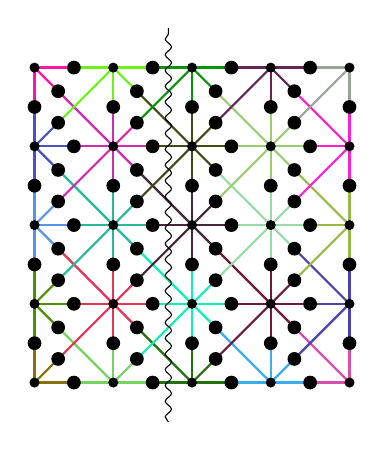
\begin{tikzpicture}
    \def\r{0.08}
    \def\a{0.07}
    \def\L{0.6}
    \def\l{0.1}
    \def\sql{0.24}
    \pgfmathsetseed{2}
    \foreach[evaluate={\cr=0.1+0.5*Mod(\x,2)}] \x in {1,...,5}
        \foreach[evaluate={\cg=0.1+0.3*Mod(\y,2); \cy=0.5-0.5*Mod(\y,2)}] \y in {1,...,5}{
            \edef\R{\pdfuniformdeviate 255}
            \edef\G{\pdfuniformdeviate 255}
            \edef\B{\pdfuniformdeviate 255}
            \xdefinecolor{MyColor}{RGB}{\R,\G,\B}
            \ifnum \x < 5
                \draw [thick, MyColor, opacity=1.0, line cap=round] (\x,\y) -- (\x+0.5,\y);
                \ifnum \y < 5
                \draw [thick, MyColor, opacity=1.0, line cap=round] (\x,\y) -- (\x+0.3,\y+0.3);
                \fi
                \ifnum \y > 1
                \draw [thick, MyColor, opacity=1.0, line cap=round] (\x,\y) -- (\x+0.3,\y-0.3);
                \fi
            \fi
            \ifnum \x > 1
                \draw [thick, MyColor, opacity=1.0, line cap=round] (\x,\y) -- (\x-0.5,\y);
                \ifnum \y < 5
                \draw [thick, MyColor, opacity=1.0, line cap=round] (\x,\y) -- (\x-0.7,\y+0.7);
                \fi
                \ifnum \y > 1
                \draw [thick, MyColor, opacity=1.0, line cap=round] (\x,\y) -- (\x-0.7,\y-0.7);
                \fi
            \fi
            \ifnum \y < 5
                \draw [thick, MyColor, opacity=1.0, line cap=round] (\x,\y) -- (\x,\y+0.5);
            \fi
            \ifnum \y > 1
                \draw [thick, MyColor, opacity=1.0, line cap=round] (\x,\y) -- (\x,\y-0.5);
            \fi
        }
    \foreach \x in {1,...,5}
        \foreach \y in {1,...,5}{
            \filldraw[fill=black] (\x,\y) circle [radius=0.7*\r];
        }
    \foreach \x in {1,...,5}
        \foreach \y in {1,...,5}{
            \ifnum \y < 5
                \filldraw[fill=black] (\x,\y+0.5) circle [radius=\r];
                \filldraw[fill=black] (\y+0.5,\x) circle [radius=\r];
            \fi
        }
    \foreach \x in {1,...,4}
        \foreach \y in {1,...,4}{
            \filldraw[fill=black] (\x+0.3,\y+0.3) circle [radius=\r];
            \filldraw[fill=black] (\y+0.3,\x+0.7) circle [radius=\r];
        }
    \tikzset{decoration={snake,amplitude=.4mm,segment length=2mm,
                    post length=0mm,pre length=0mm}}
    \draw [decorate] (2.7, 0.5) -- (2.7, 5.5);
\end{tikzpicture}}
where we use different colors to distinguish different hyperedges.
Now, the vertex tensor is always rank $1$.
With the same naive contraction order, we can see the maximum intermediate tensor is approximately of size $2^L$ by counting the colors.

\section{Generalizing to other graph problems}\label{app:otherproblems}
There are some other graph problems that can be encoded in a tensor network.
To understand its representation power, it is a good starting point to connect it with dynamic programming because
a tensor network can be viewed as a special type of dynamic programming where its update rule can be characterized by a linear operation.
Courcelle’s theorem~\cite{Courcelle1990,Barr2020} states that a problem quantified by monadic second order logic (MSO) on a graph with bounded treewidth $k$ can be solved in linear time with respect to the graph size.
Dynamic programming is a traditional approach to attack a MSO problem, it can solve the maximum independent set problem in $O(2^k)n$, which is similar to the tensor network approach.
We mentioned in the main text that tensor network has nice analytic property make it easier for generic programming.
The cost is, the tensor network is less expressive than dynamic programming,
%\iffalse
%The cost is, it is less expressive than MSO because the tensor network described by \Eq{eq:tensor} can be expressed in MSO as
%\begin{align}
%    \begin{split}
%    \exists_X\forall_{u}&(\\
%    &\quad\forall_{v} 
%    \neg {\rm adj}(u, v) \lor
%    ({\rm adj}(u, v) \land ( \hspace{5em}\text{$\triangleright$ restrictions on edges}\\
%    &\quad\quad(u \not\in X \land v \not\in X \land B_{00}) \lor\\
%    &\quad\quad(u \not\in X \land v \in X \land B_{01}) \lor\\
%    &\quad\quad(u \in X \land v \not\in X \land B_{10}) \lor\\
%    &\quad\quad(u \in X \land v \in X \land B_{11})\\
%    &\quad)\\
%    &))\land\\
%    &(\hspace{16.5em}\text{$\triangleright$ restrictions on vertices}\\
%    &\quad(u \not\in X \land W_{0}) \lor\\
%    &\quad(u \in X \land W_{1})\\
%    &),
%    \end{split}
%\end{align}
%while not all monadic second order logic can be represented as a tensor network contraction,
%for example, it is hard to construct a tensor network to decide whether a graph is connected or not.
%At the cost of losing expressiveness, we can encode the properties of the graph into the tensor elements.
%\fi
However, that are still some other problems that can be expressed in the framework of generic tensor network.
\subsection{Matching problem}
A matching polynomial of a graph $G$ is defined as
\begin{equation}
    M(G, x) = \sum\limits_{k=1}^{|V|/2} c_k x^k,
\end{equation}
where $k$ is the number of matches, and coefficients $c_k$ are the corresponding counting.

We define a tensor of rank $d(v) = |N(v)|$ on vertex $v$ such that,
\begin{equation}
    W_{v\rightarrow n_1, v\rightarrow n_2, \ldots, v\rightarrow n_{d(v)}} = \begin{cases}
        1, & \sum_{i=1}^{d(v)} v\rightarrow n_i \leq 1,\\
        0, & \text{otherwise},
    \end{cases}
\end{equation}
and a tensor of rank $1$ on the bond
\begin{equation}
    B_{v\rightarrow w} = \begin{cases}
    1, & v \rightarrow w = 0 \\
    x, & v \rightarrow w = 1.
\end{cases}
\end{equation}
Here, we use bond index $v \rightarrow w$ to label tensors.

\subsection{k-Coloring}
Let us use 3-coloring on the vertex as an example. We can define a vertex tensor as
\begin{equation}
    W = \left(\begin{matrix}
        r_v\\
        g_v\\
        b_v
    \end{matrix}\right),
\end{equation}
and an edge tensor as
\begin{equation}
    B = \left(\begin{matrix}
        0 & 1 & 1\\
        1 & 0 & 1\\
        1 & 1 & 0
    \end{matrix}\right).
\end{equation}
The number of possible coloring can be obtained by contracting this tensor network by setting vertex tensor elements $r_v, g_v$ and $b_v$ to $1$.
By designing generic types as tensor elements, one should be able to get all possible colorings.
It is straight forward to define the k-coloring problem on edges hence we will not discuss the detailed construction here.

\subsection{Max cut problem}
Max cut problem is also known as the boolean spinglass problem.
Its tensor network representation does not contain vertex tensors.
The edge tensor can be defined as
\begin{equation}
    B(x_{ij}) = \left(\begin{matrix}
        1 & x_{ij}\\
        x_{ij} & 1
    \end{matrix}\right).
\end{equation}
We can also define a polynomial about edges variables by setting $x_{ij} = x$,
its $k$th coefficient is two times the number of configurations of cut size $k$.

\subsection{Set packing}
Set packing the the hypergraph version of the maximum independent set problem, where each set corresponds to a vertex, each element corresponds to a hyperedge.
To solve the set packing problem, we just remove the rank 2 restriction of an edge tensor
\begin{equation}
    B_{v,w,\ldots, z} = \begin{cases}
        1, & v+w+\ldots+z\leq 1,\\
        0, & otherwise
    \end{cases}
\end{equation}

\section{Discrete Fourier transform for computing the independence polynomial}\label{app:fft}

In section~\ref{sec:indpoly}, we show that the independence polynomial can be obtained by solving the linear equation \Eq{eq:lineareq}. Since the coefficients of the independence polynomial can range many orders of magnitude, the round-off errors in fitting can be significant if we use random floating point numbers for $x_{i}$.
In the main text, we propose to use a finite field $\text{GF}(p)$ to circumvent overflow and round-off errors. Here, we give another method based on discrete Fourier transform.
Instead of choosing $x_{i}$ as random numbers, we can choose them such that they form a geometric sequence in the complex domain $x_j = r\omega^j$, where $r \in \mathbb{R}$ and $\omega = e^{-2\pi i/( \alpha(G)+1)}$. The linear equation thus becomes
\begin{equation}
\left(\begin{matrix}
1 & r & r^2 & \ldots & r^{\alpha(G)} \\
1 & r\omega & r^2\omega^2 & \ldots & r^{\alpha(G)} \omega^{\alpha(G)} \\
\vdots & \vdots & \vdots &\ddots & \vdots \\
1 & r\omega^{\alpha(G)} & r^2\omega^{2{\alpha(G)}} & \ldots & r^{\alpha(G)}\omega^{{\alpha(G)}^2}
\end{matrix}\right)
\left(\begin{matrix}
a_0 \\ a_1 \\ \vdots \\ a_{\alpha(G)}
\end{matrix}\right)
= \left(\begin{matrix}
y_0 \\ y_1 \\ \vdots \\ y_{\alpha(G)}
\end{matrix}\right).
\end{equation}

Let us rearrange the coefficients $r^j$ to $a_j$, the matrix on the left side becomes the discrete Fourier transform matrix. Thus, we can obtain the coefficients by inverse Fourier transform $\vec a_r = {\rm FFT^{-1}}(\omega) \cdot \vec y$, where $(\vec a_r)_j = a_j r ^j$.
By choosing different $r$, one can obtain better precision in low independent set size region  ($r<1$) or high independent set size region ($r>1$).

\section{Integer sequences formed by the number of independent sets}

\begin{table}[h]
\caption{The number of independent sets for square grid graphs of size $L\times L$. This forms the integer sequence \href{https://oeis.org/A006506}{OEIS A006506}.}
\begin{center}
\scalebox{0.9}{
\begin{tabular}{|c| >{\centering\arraybackslash} p{0.95\linewidth}|}
 \hline $L$  & square grid graphs \\
 \hline $ 1$ & 2  \\
 \hline $ 2$ & 7  \\
 \hline $ 3$ & 63  \\
 \hline $ 4$ & 1 234  \\
 \hline $ 5$ & 55 447  \\
 \hline $ 6$ & 5 598 861  \\
 \hline $ 7$ & 1 280 128 950  \\
 \hline $ 8$ & 660 647 962 955  \\
 \hline $ 9$ & 770 548 397 261 707  \\
 \hline $ 10$ & 2 030 049 051 145 980 050  \\
 \hline $ 11$ & 12 083 401 651 433 651 945 979  \\
 \hline $ 12$ & 162 481 813 349 792 588 536 582 997  \\
 \hline $ 13$ & 4 935 961 285 224 791 538 367 780 371 090  \\
 \hline $ 14$ & 338 752 110 195 939 290 445 247 645 371 206 783  \\
 \hline $ 15$ & 52 521 741 712 869 136 440 040 654 451 875 316 861 275  \\
 \hline $ 16$ &  18 396 766 424 410 124 752 958 806 046 933 947 217 821 482 942 \\
 \hline $ 17$ &  14 557 601 701 834 111 295 974 187 104 248 827 765 798 599 152 358 303 \\
 \hline $ 18$ &  26 024 585 612 650 837 861 658 126 921 792 857 026 992 497 268 285 945 167 621 \\
 \hline $ 19$ &  105 105 055 066 577 962 012 604 229 608 317 915 229 737 651 637 019 975 757 755 051 314 \\
 \hline $ 20$ &  958 979 036 662 929 619 406 859 624 886 958 746 851 620 546 557 485 230 898 539 651 354 907 499 \\
 \hline $ 21$ &  19 766 982 580 727 525 559 447 459 703 066 410 506 378 295 841 376 040 664 015 562 851 325 369 819 076 327 \\
 \hline $ 22$ &  920 486 427 724 231 647 653 646 535 134 255 190 048 558 085 587 696 509 535 085 179 014 710 020 739 303 637 413 062 \\
 \hline $ 23$ & 96 836 737 362 332 577 228 126 233 146 266 027 907 220 602 904 916 569 863 928 397 932 638 147 313 462 817 836 132 159 477 643 \\
 \hline $ 24$ & 23 014 876 830 102 973 080 295 375 510 481 185 265 791 418 130 718 634 637 816 237 986 620 978 856 344 595 418 898 906 840 911 239 867 869 \\
 \hline $ 25$ & 12 357 280 628 458 621 610 261 003 683 798 282 889 567 362 022 871 449 310 490 079 744 330 288 088 293 888 381 458 751 196 205 785 114 467 063 479 978 \\
 \hline $ 26$ & 14 989 353 830 657 887 045 253 535 577 369 170 604 561 059 504 403 111 230 207 533 142 521 161 755 543 754 839 412 836 401 335 298 693 619 461 437 872 472 165 615 \\
 \hline $ 27$ &  41 076 048 814 756 904 170 038 431 958 637 474 710 328 322 517 168 428 037 124 975 797 939 221 729 929 250 098 889 601 666 346 169 376 778 430 801 983 574 787 538 529 309 191 \\
 \hline $ 28$ &  254 296 368 874 677 123 746 928 211 898 730 495 474 495 246 876 690 760 159 507 126 754 738 599 026 016 292 991 448 162 576 157 292 681 301 528 315 863 006 160 203 433 527 765 235 617 478 \\
 \hline $ 29$ & 3 556 619 491 488 838 337 298 644 336 171 591 528 960 687 731 348 622 394 588 805 214 244 031 766 315 339 709 627 465 589 460 212 852 431 000 227 410 783 701 037 177 097 019 793 172 369 009 198 594 591 \\
 \hline $ 30$ &  112 377 766 778 527 126 203 646 648 402 050 958 984 330 252 199 994 469 198 044 986 979 798 657 215 652 532 005 142 877 926 040 203 499 014 641 860 333 039 219 325 350 361 465 468 647 055 420 204 598 509 312 491 705 \\
  \hline
\end{tabular}
}
\end{center}
\label{tbl:squaregrid}
\end{table}


\begin{table}[h]
\caption{The number of independent sets for King's graphs of size $L\times L$.}
\begin{center}
\begin{tabular}{|c| >{\centering\arraybackslash} p{0.85\linewidth}|}
 \hline $L$  & King's graphs \\
 \hline $ 1$ & 2  \\
 \hline $ 2$ & 5  \\
 \hline $ 3$ & 35  \\
 \hline $ 4$ & 314 \\
 \hline $ 5$ & 6 427 \\
 \hline $ 6$ & 202 841 \\
 \hline $ 7$ & 12 727 570  \\
 \hline $ 8$ & 1 355 115 601 \\
 \hline $ 9$ & 269 718 819 131 \\
 \hline $ 10$ & 94 707 789 944 544 \\
 \hline $ 11$ & 60 711 713 670 028 729  \\
 \hline $ 12$ & 69 645 620 389 200 894 313  \\
 \hline $ 13$ &  144 633 664 064 386 054 815 370 \\
 \hline $ 14$ & 540 156 683 236 043 677 756 331 721  \\
 \hline $ 15$ & 3 641 548 665 525 780 178 990 584 908 643  \\
 \hline $ 16$ & 44 222 017 282 082 621 251 230 960 522 832 336 \\
 \hline $ 17$ & 968 503 939 616 343 947 563 582 929 715 005 880 647 \\
 \hline $ 18$ & 38 227 887 218 717 761 202 510 261 178 854 062 185 464 315 \\
 \hline $ 19$ & 2 720 444 488 584 821 384 410 936 779 813 343 554 469 758 172 682 \\
 \hline $ 20$ & 348 970 226 122 589 397 373 342 369 495 005 120 745 703 462 667 115 175 \\
 \hline $ 21$ & 80 700 603 403 721 730 646 640 814 391 653 008 712 705 595 500 769 624 448 529 \\
 \hline $ 22$ & 33 641 616 174 796 469 294 898 513 022 199 100 689 671 634 779 118 656 571 910 751 320 \\
 \hline $ 23$ & 25 281 578 706 433 684 460 290 055 263 926 749 952 595 755 044 481 112 956 327 672 312 862 611  \\
 \hline $ 24$ & 34 249 181 078 331 384 968 700 380 345 306 575 903 108 280 266 841 066 358 396 857 518 201 026 192 547 \\
 \hline $ 25$ & 83 641 072 313 734 275 009 578 098 702 552 656 178 287 685 025 530 905 558 603 555 359 601 823 180 929 638 318  \\
 \hline $ 26$ & 368 222 048 967 797 645 785 624 418 568 072 838 671 415 214 857 177 141 161 824 615 541 365 640 076 045 923 328 316 979  \\
 \hline $ 27$ & 2 922 282 601 123 898 422 508 409 690 495 824 015 239 663 506 989 438 099 254 205 806 998 557 618 858 143 959 252 475 337 777 029  \\
 \hline $ 28$ & 41 807 680 908 633 213 277 041 952 346 680 116 482 996 387 928 973 684 599 097 559 098 879 721 953 006 036 791 335 134 446 016 561 667 772 \\
  \hline
\end{tabular}
\end{center}
\label{tbl:kingsgrid}
\end{table}

We also computed independence polynomial rigorously for these lattices in our Github repo\blue{add link to the repo}.

\end{document}
